\documentclass[a4paper,12pt]{report}
\usepackage[left=3cm,right=2.5cm,top=2.5cm,bottom=2.5cm]{geometry}
\usepackage[T1]{fontenc}
\usepackage[utf8]{inputenc}
\usepackage[english,greek]{babel}
\usepackage{amsmath,amsfonts,amssymb,amsthm}
\usepackage[parfill]{parskip}
\usepackage[unicode]{hyperref}
\usepackage{bookmark}
\usepackage{cite}
\usepackage{graphicx}
\usepackage{wrapfig}
\usepackage{subcaption}
\usepackage{float}
\usepackage{siunitx}
\usepackage{color}
\usepackage{kmath,kerkis}
\usepackage{url}
\usepackage{hyperref}
\usepackage{tikz}
\usepackage[ruled,nosemicolon,linesnumbered]{algorithm2e}
\let\oldnl\nl% Store \nl in \oldnl
\newcommand{\nonl}{\renewcommand{\nl}{\let\nl\oldnl}}% Remove line number for one line


\graphicspath{{../graphics/}}

\def\tl{\textlatin}
\def\tg{\textgreek}

\newtheorem{definition}{Ορισμός}
\newtheorem{lemma}{Λήμμα}

\def\bigO{\mathcal{O}}

\begin{document}

\begin{titlepage}

\begin{figure}[H]
  \begin{center}
    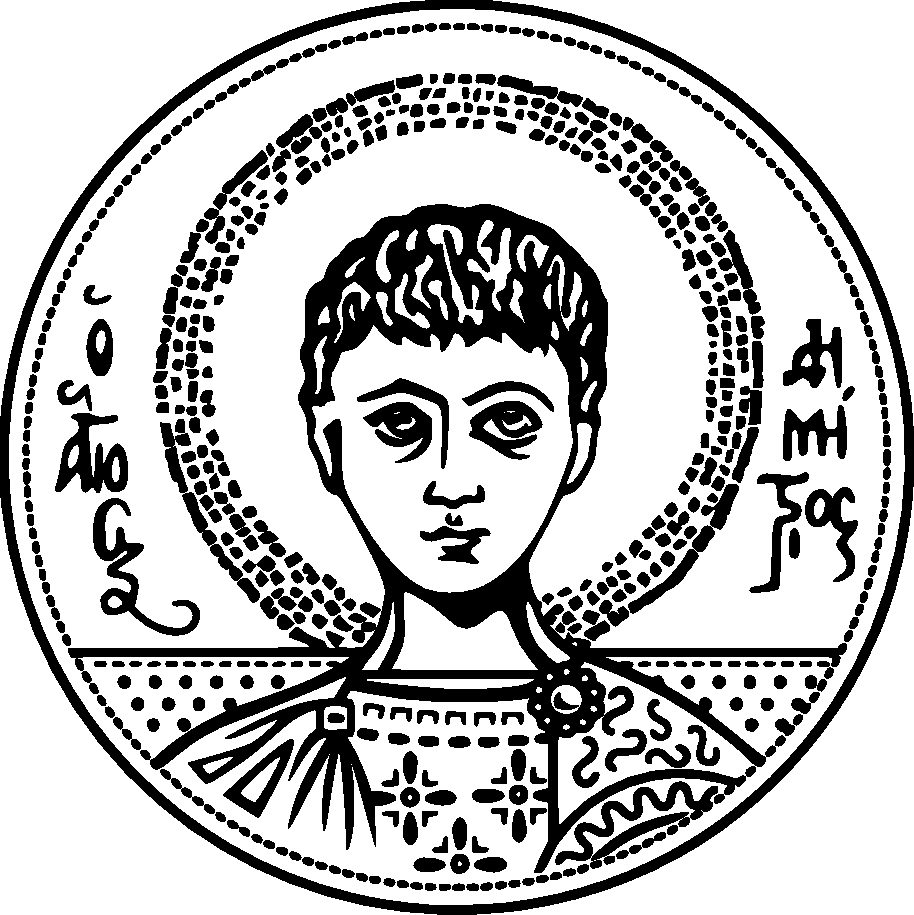
\includegraphics[width=3cm]{auth.pdf}
    \label{fig:cover_auth_logo}
  \end{center}
\end{figure}

\centering
\Large Αριστοτέλειο Πανεπιστήμιο Θεσσαλονίκης\\
\Large Πολυτεχνική Σχολή\\
\large Τμήμα Ηλεκτρολόγων Μηχανικών και Μηχανικών Υπολογιστών\\
\large Τομέας Ηλεκτρονικής και Υπολογιστών

\vspace{\fill}

\LARGE Υπολογισμός της Ευκλείδειας Απόστασης δύο Τριγωνικών Πλεγμάτων

\vspace{\fill}

\Large Διπλωματική Εργασία\\
\Large Καρελής Παναγιώτης

\vspace{\fill}
\raggedright

\begin{tabular}{ll}
\textbf{Επιβλέπων:} & Πιτσιάνης Νικόλαος\\
 & Αναπληρωτής Καθηγητής Α.Π.Θ.\\
\end{tabular}

\centering
\vspace{\fill}
\today

\end{titlepage}

\begin{abstract}
Σε μια πληθώρα εφαρμογών της Υπολογιστικής Γεωμετρίας 
(Μηχανική με τη Βοήθεια Υπολογιστών (\tl{CAE}), Προσομοιώσεις με Υπολογιστές, 
Ρομποτική, Γραφική με Υπολογιστές κ.α.)
τα αντικείμενα του χώρου αναπαρίστανται συνήθως από 
πολυγωνικά πλέγματα.
Κοινό πρόβλημα για όλους τους παραπάνω τομείς αποτελεί η εύρεση της
απόστασης που διαχωρίζει δύο αντικείμενα και η ανίχνευση σύγκρουσης
μεταξύ τους.
Στην παρούσα εργασία, προτείνουμε αποδοτικούς αλγορίθμους που υπολογίζουν 
την Ευκλείδεια απόσταση δύο αντικειμένων του τρισδιάστατου χώρου και τους υλοποιούμε 
για την περίπτωση των τριγωνικών πλεγμάτων. 
Για τους αλγορίθμους αυτούς σχεδιάζουμε μια δενδρική δομή δεδομένων που
ανήκει στην κατηγορία των Ιεραρχιών Οριoθετικών Όγκων (\tl{BVH}).
Η διαδικασία κατασκευής της παραπάνω δομής είναι παρόμοια με αυτή
του \tl{KD-Tree}, με τη διαφορά ότι η δομή μας διαχειρίζεται
χωρικά δεδομένα και κάνει χρήση 
Οριοθετικών Πλαισίων Ευθυγραμμισμένων με τους Άξονες (\tl{AABB}). 
Επιπλέον, περιγράφουμε έναν τρόπο διάσχισης της δομής ώστε να
υποστηρίζει ερωτήματα κοντινότερου γείτονα για χωρικά δεδομένα.
Η διάσχιση της δενδρικής δομής σχεδιάζεται ως μια κατευθυνόμενη 
αναζήτηση κατά βάθος (\tl{DFS}), που στοχεύει στη σμίκρυνση του 
χώρου αναζήτησης μέσω κλαδέματος του δένδρου κατά την 
οπισθοδρόμηση. 
Ακόμη, στην υλοποίηση μας παραλληλοποιούμε τη διαδικασία
κατασκευής του δένδρου όπως και τη διαδικασία αναζήτησης της ελάχιστης 
απόστασης κάνοντας χρήση πολλαπλών νημάτων επεξεργασίας. 
Τέλος, μετράμε και αναλύουμε την επίδοση των αλγορίθμων μας σε μια σειρά
από περιπτώσεις ελέγχου που κατασκευάσαμε. 

\textbf{Λέξεις-κλειδιά:} \\
\textit{Υπολογιστική Γεωμετρία, Πολυγωνικά Πλέγματα, Ευκλείδεια Απόσταση,
Ιεραρχίες Οριοθετικών Όγκων}
\end{abstract}

\selectlanguage{english}
\begin{abstract}
In a plethora of fields in Computational Geometry 
(Computer Aided Engineering, Computer Simulations,
Robotics, Computer Graphics etc.) objects in space are 
represented as polygonal meshes.
A common problem, for all the above, is the computation of
separation distance and collision detection of two objects.
In this thesis, we propose efficient algorithms that compute 
the Euclidean distance of two objects in 3D space and we implement
them for the case of triangle meshes.
For these algorithms we design a tree data structure that 
belongs to the family of Bounding Volume Hierarchies (BVH).
The construction procedure of this data structure is similar
to the one used by the KD-Tree, but it differs, as our data 
structure manages spatial data and also uses Axis-Aligned 
Bounding Boxes (AABB).
In addition, we describe a traversal scheme of the data 
structure in order to answer nearest neighbor queries 
for spatial data.
The traversal of the tree structure is implemented 
as a directed depth first search (DFS), aiming to reduce 
the searching space by pruning the tree during backtracking.
Furthermore, we parallelize the construction of the data 
structure as well as the procedure of finding the Euclidean
distance, using multithreading.
Finally, we measure and analyze the efficiency of our 
algorithms on a series of test cases we created.

\textbf{Keywords:} \\
\textit{Computational Geometry, Polygonal Meshes, Euclidean Distance,
Bounding Volumes Hierarchies}

\end{abstract}

\thispagestyle{empty}

\selectlanguage{greek}

\section*{Ευχαριστίες}
\thispagestyle{empty}

Με την παρούσα διπλωματική εργασία ολοκληρώνω τις σπουδές μου 
στο τμήμα Ηλεκτρολόγων Μηχανικών και Μηχανικών Η/Υ του Α.Π.Θ. 
Θα ήθελα να ευχαριστήσω τον καθηγητή μου Νικόλαο Πιτσιάνη 
όχι μόνο για τις γνώσεις που μου παρείχε αυτά τα χρόνια, αλλά 
και για την καταλυτική συνδρομή του στο να ανακαλύψω τα ενδιαφέροντα 
μου μέσα στο ευρύ φάσμα δραστηριοτήτων ενός μηχανικού υπολογιστών.

Ευχαριστώ τους γονείς μου Βασίλη και Νίκη καθώς και την αδερφή μου 
Δήμητρα, για τη συμπαράσταση τους σε όλο αυτό το ταξίδι και για την εμπιστοσύνη 
που μου έδειξαν από την πρώτη στιγμή.

Πολλά ευχαριστώ στον φίλο μου, και συνάδελφο, Μανώλη, που με βοήθησε να 
εξελιχθώ σε όλους τους τομείς της ζωής μου.

Ευχαριστώ την οικογένεια Καραγεωργίου, η οποία στάθηκε δίπλα μου σαν 
δεύτερη οικογένεια.
Ιδιαίτερα ευχαριστώ τον Λάζαρο και τον Ιωσήφ, που με τον τρόπο τους, 
με βοήθησαν να βελτιωθώ και έπαιξαν σημαντικό ρόλο στις αποφάσεις 
που πήρα μέχρι τώρα και στις αποφάσεις που θα πάρω στο μέλλον.

Τέλος, ευχαριστώ όλους τους φίλους, συναδέλφους και γνωστούς που πέρασα 
μαζί τους στιγμές τις οποίες θα θυμάμαι για πάντα,
όταν θα σκέφτομαι τα φοιτητικά μου χρόνια.


\clearpage


\title{Υπολογισμός της Ευκλείδειας Απόστασης δύο Τριγωνικών Πλεγμάτων}
\author{Παναγιώτης Καρελής \\
\href{mailto:karelisp@ece.auth.gr}{\tl{karelisp@ece.auth.gr}}}
\maketitle

\tableofcontents
\thispagestyle{empty}

\chapter{Εισαγωγή}
\label{ch:introduction}
\section{Κίνητρο}

\section{Περιγραφή του Προβλήματος}

\section{Στόχοι της Διπλωματικής Εργασίας}

\section{Διάρθρωση της Διπλωματικής Εργασίας}
Στο \textbf{Κεφάλαιο \ref{ch:introduction}} έγινε μια εισαγωγή στο 
πρόβλημα υπολογισμού της απόστασης δύο πλεγμάτων και παρουσιάστηκαν
τα κίνητρα που οδήγησαν στην υλοποίηση των αλγορίθμων που θα 
παρουσιαστούν. 

Στο \textbf{Κεφάλαιο \ref{ch:theoretical_background}} παρουσιάζεται το 
θεωρητικό υπόβαθρο που απαιτείται από τον αναγνώστη ώστε να κατανοήσει
πλήρως το πρόβλημα και την προτεινόμενη λύση.

Στο \textbf{Κεφάλαιο \ref{ch:related_work}} αναφέρεται η σχετική 
βιβλιογραφία, δηλαδή πώς αντιμετώπισαν άλλοι ερευνητές το ίδιο ή 
παρόμοια προβλήματα. 
Παρουσιάζονται επίσης ομοιότητες και διαφορές
των υπολοίπων προσεγγίσεων σε σχέση με τη δική μας.

Στο \textbf{Κεφάλαιο \ref{ch:methodology}} αναλύεται η μεθοδολογία 
που προτείνουμε και παρουσιάζεται η υλοποίηση των αλγορίθμων μας.

Στο \textbf{Κεφάλαιο \ref{ch:experiments}} παρατίθενται τα αποτελέσματα 
από τα πειράματα που εκτελέσαμε. 
Οι μετρήσεις των πειραμάτων περιλαμβάνουν την εκτίμηση της συνάρτησης 
κόστους που ορίζεται στην ενότητα \ref{sec:cost_metric} καθώς και τους χρόνους
εκτέλεσης των αλγορίθμων. 

Στο \textbf{Κεφάλαιο \ref{ch:future_work}} σχολιάζονται τα αποτελέσματα
και παρουσιάζονται σκέψεις για μελλοντική επέκταση και βελτίωση των 
ιδεών της παρούσας διπλωματικής εργασίας.

\chapter{Θεωρητικό Υπόβαθρο}
\label{ch:theoretical_background}

\section{Πλέγματα}
\begin{wrapfigure}{r}{0.25\textwidth}
    \centering
    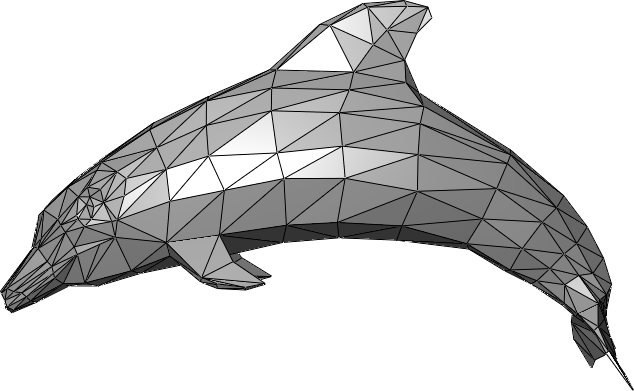
\includegraphics[width=0.25\textwidth]{Dolphin_triangle_mesh.png}
    \caption[Παράδειγμα Τριγωνικού Πλέγματος]{
        Παράδειγμα τριγωνικού πλέγματος που αναπαριστά ένα δελφίνι.
    }
    \label{fig:example_mesh}
\end{wrapfigure}
\label{sec:triangle_meshes}
Στην Υπολογιστική Γεωμετρία τα \textit{πλέγματα} αποτελούν την αναπαράσταση
μιας μεγαλύτερης γεωμετρικής περιοχής από μικρότερα διακριτά στοιχεία.
Τα πλέγματα χρησιμοποιούνται συνήθως για τον υπολογισμό λύσεων μερικών 
διαφορικών εξισώσεων, για την απόδοση γραφικών υπολογιστών, και για
ανάλυση γεωγραφικών και χαρτογραφικών δεδομένων.
Ένα πλέγμα χωρίζει τον χώρο σε μικρότερα στοιχεία (πολύγωνα ή πολύεδρα) όπου
μπορούν να λυθούν οι εξισώσεις, το οποίο στη συνέχεια προσεγγίζει τη λύση 
στο ευρύτερο πεδίο. 
Τα πλέγματα που αποτελούνται από πολύεδρα αντιπροσωπεύουν ρητά τόσο την 
επιφάνεια όσο και τον όγκο ενός αντικειμένου, ενώ τα πολυγωνικά 
πλέγματα αντιπροσωπεύουν μόνο την επιφάνεια (ο όγκος υπονοείται).
Για το πρόβλημα υπολογισμού της Ευκλείδειας απόστασης, ενδιαφερόμαστε 
μόνο για την εξωτερική επιφάνεια των αντικειμένων του τρισδιάστατου χώρου. 

Ένας τύπος πολυγωνικών πλεγμάτων είναι τα τριγωνικά πλέγματα 
(σχήμα \ref{fig:example_mesh}).
Αποτελούνται από ένα σύνολο τριγώνων στις τρεις διαστάσεις, 
τα οποία συνδέονται με τις κοινές τους ακμές ή κορυφές. 
Γεωμετρικά, ένα πλέγμα είναι μια τμηματικά επίπεδη επιφάνεια.
Η τελευταία ιδιότητα ισχύει πάντοτε για τα τριγωνικά πλέγματα.

Υπάρχουν διάφοροι τρόποι για την αποθήκευση ενός τριγωνικού πλέγματος 
στη μνήμη του υπολογιστή. 
Υπάρχουν επίσης μέθοδοι μετατροπής του ενός 
τρόπου αποθήκευσης σε έναν άλλο.
Ενδεικτικά αναφέρουμε την αποθήκευση με:
\begin{itemize}
    \item \textbf{Σετ τριγώνων}: 
    Το πλέγμα αναπαρίσταται απλά από τα τρίγωνα 
    του. 
    Δηλαδή αποθηκεύονται οι συντεταγμένες των κορυφών κάθε τριγώνου.
    \item \textbf{Σετ Τριγώνων με δείκτες}: 
    Το πλέγμα αναπαρίσταται από ένα σετ
    κόμβων και ένα σετ από τριπλέτες με δείκτες στους κόμβους.
    Η κάθε τριπλέτα αναπαριστά ένα τρίγωνο.
    \item \textbf{Λωρίδες Τριγώνων}: 
    Η αποθήκευση αυτή βασίζεται στο γεγονός ότι 
    δύο γειτονικά τρίγωνα μοιράζονται τη μία τους πλευρά. Αυτός 
    ο τρόπος χρησιμοποιείται για συμπίεση των πλεγμάτων.
    \item \textbf{Δομή Τρίγωνου-Γείτονα}: 
    Υποστηρίζει ερωτήματα γειτνίασης τριγώνων.
    \item \textbf{Δομή \tl{Winged-Edge}}: 
    Αποθηκεύει δεδομένα κόμβων, ακμών και όψεων.
    Επιτρέπει εύκολη διάβαση στο πλέγμα μεταξύ όψεων, ακμών και κορυφών.
\end{itemize} 
Για τους αλγορίθμους που περιγράφουμε παρακάτω αρκεί ο πρώτος τρόπος 
αναπαράστασης. 

Τέλος, για τις διάφορες εφαρμογές που χρησιμοποιούνται, τα πλέγματα 
χαρακτηρίζονται και από την ποιότητα τους. Οι πιο συνηθισμένες μετρικές 
ποιότητας είναι:
\begin{itemize}
    \item \textbf{Λοξότητα (\tl{Skewness})}: \\
    Η λοξότητα είναι ο λόγος της απόκλισης μεταξύ του βέλτιστου μεγέθους
    στοιχείου προς στο υπάρχον μέγεθος στοιχείου. 
    Το εύρος της λοξότητας είναι μεταξύ 0 (ιδανικό) έως 1 (χειρότερο).
    Τα πολύ λοξά στοιχεία δεν προτιμώνται λόγω της κακής ακρίβειας 
    που προκαλούν στις παρεμβαλλόμενες περιοχές.
    Ανάλογα με το στοιχείο (τρίγωνο, τετράπλευρο, τετράεδρο, 
    εξάεδρο κλπ) διαφοροποιείται μαθηματικός τύπος 
    για τον υπολογισμό της λοξότητας.

    \item \textbf{Ομαλότητα (\tl{Smoothness})}: \\
    Η αλλαγή στο μέγεθος των στοιχείων πρέπει να είναι ομαλή. 
    Συνήθως αποφεύγονται ξαφνικά άλματα στο μέγεθος των στοιχείων γιατί αυτό 
    μπορεί να προκαλέσει λανθασμένα αποτελέσματα σε κοντινούς κόμβους.
    
    \item \textbf{Αναλογία Διαστάσεων (\tl{Aspect Ratio})}: \\
    Εν συντομία, ο λόγος διαστάσεων είναι ο λόγος του μεγαλύτερου μήκους 
    ενός στοιχείου προς το μικρότερο μήκος. 
    Ο ιδανικός λόγος διαστάσεων είναι 1. 
    Όσο μικρότερος είναι, τόσο υψηλότερη είναι η ποιότητα ενός στοιχείου. 
    Η μέθοδος υπολογισμού ποικίλλει ανάλογα με τον τύπο κελιού.
\end{itemize}

Σε ρεαλιστικές εφαρμογές, τα πλέγματα συνήθως σχεδιάζονται έτσι ώστε 
να μην παραβιάζουν σε μεγάλο βαθμό τις παραπάνω μετρικές ποιότητας.
Αυτή η παρατήρηση είναι χρήσιμη για τον σχεδιασμό της δομής δεδομένων 
που προτείνουμε.

\begin{figure}[h]
    \centering
    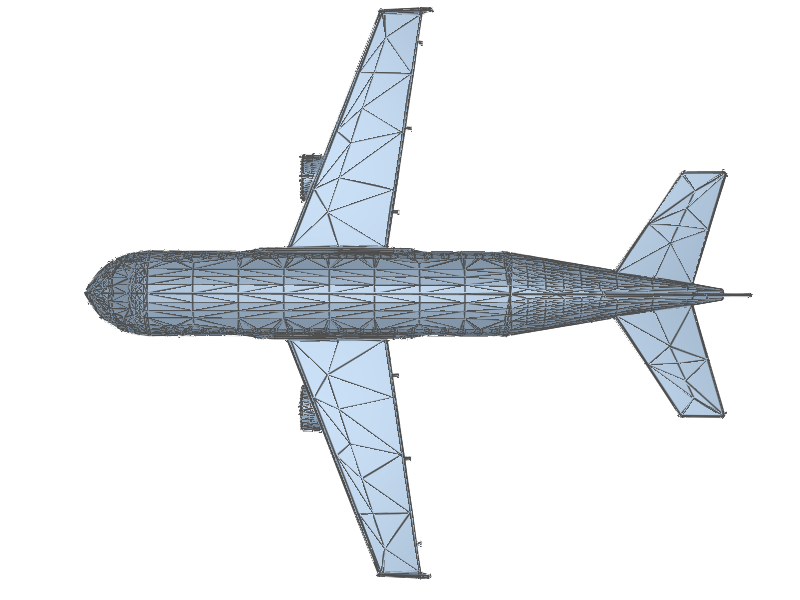
\includegraphics[width=0.45\textwidth]{airplane_bad_mesh.png}
    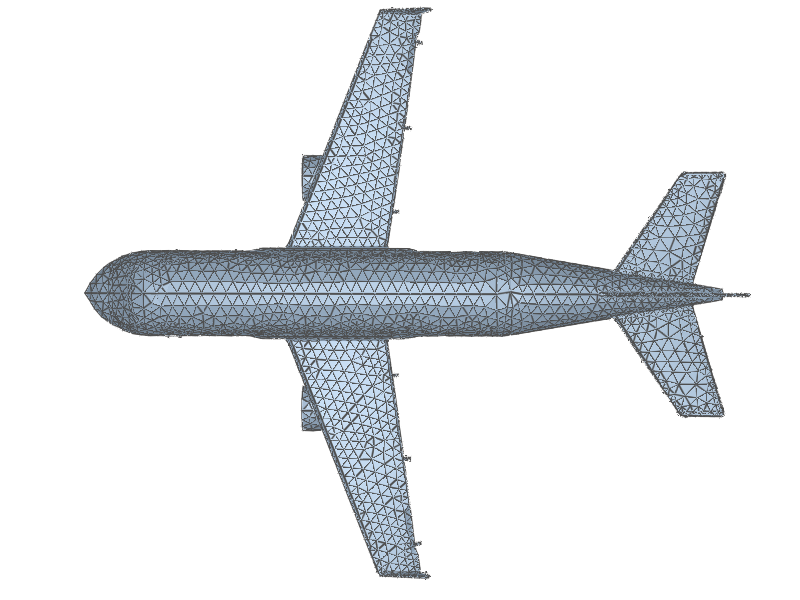
\includegraphics[width=0.45\textwidth]{airplane_good_mesh.png}
    \caption[Παράδειγμα Ποιότητας Πλεγμάτων]{
        Παράδειγμα Ποιότητας Πλεγμάτων - Και τα δύο πλέγματα 
        αναπαριστούν το ίδιο αεροπλάνο. Το δεξί πλέγμα είναι 
        καλύτερης ποιότητας από το αριστερό που φαίνεται να 
        παραβιάζει όλα τα κριτήρια ποιότητας που αναφέρθηκαν
        (\tl{skweness, smoothness, aspect ratio}). Και τα 
        δύο πλέγματα αποτελούνται από τον ίδιο αριθμό τριγώνων
        περίπου (γύρω στα $15000$ τρίγωνα).
    }
\end{figure}

\section{Οριοθετικοί Όγκοι}
\label{sec:bounding_volumes}
\textit{Οριοθετικός όγκος} (\textbf{\tl{bounding volume}}) ενός συνόλου 
από αντικείμενα του τρισδιάστατου χώρου ονομάζεται οποιοσδήποτε 
κλειστός όγκος που εξ' ολοκλήρου περικλείει τα αντικείμενα του συνόλου. 
Οι οριοθετικοί όγκοι χρησιμοποιούνται για να επιταχύνουν αλγορίθμους   
που εκτελούν γεωμετρικούς ελέγχους χρησιμοποιώντας απλούς όγκους 
που περικλείουν πολύπλοκα αντικείμενα.
Οι έλεγχοι σε οριοθετικούς όγκους είναι τυπικά πολύ ταχύτεροι από 
ελέγχους στο ίδιο το στοιχείο ή αντικείμενο που περικλείουν 
Σε πολλές περιπτώσεις, ένας έλεγχος αρκεί για να απορριφθούν ή 
να επιβεβαιωθούν πολλαπλοί έλεγχοι που θα απαιτούνταν για κάθε ένα 
από τα στοιχεία ξεχωριστά.

Οι οριοθετικοί όγκοι βρίσκουν ευρεία εφαρμογή στους παρακάτω τομείς:
\begin{itemize}
    \item \textbf{Ανίχνευση Ακτίνων (\tl{Ray Tracing})}:\\
    Oι οριοθετικοί όγκοι χρησιμοποιούνται σε ελέγχους τομής ακτίνων 
    με αντικείμενα και σε πολλούς αλγόριθμους απόδοσης γραφικών.
    Για παράδειγμα, εάν η ακτίνα ή το οπτικό πεδίο της κάμερας
    δεν τέμνει τον οριοθετικό όγκο, τότε δεν μπορεί να τέμνει ούτε 
    το αντικείμενο που περιέχεται μέσα. Έτσι αποφεύγονται οι 
    αντίστοιχοι έλεγχοι, οι οποίοι κοστίζουν υπολογιστικά.
    Όμοια, εάν το οπτικό πεδίο της κάμερας περιέχει εξ ολοκλήρου 
    τον οριοθετικό όγκο, το αντικείμενο, δηλαδή τα στοιχεία από τα
    οποία αποτελείται θα απεικονιστούν στην 
    οθόνη χωρίς περισσότερους ελέγχους. 
    
    \item \textbf{Ανίχνευση Σύγκρουσης (\tl{Collision Detection})}:\\
    Όμοια με πριν, όταν δύο οριοθετικοί όγκοι δε συγκρούονται/τέμνονται, 
    τότε ούτε και τα αντικείμενα που περικλείουν δεν μπορούν να συγκρούονται.
\end{itemize}

Για τη δημιουργία οριοθετικών όγκων σύνθετων αντικειμένων, συνήθως 
χρησιμοποιούνται \textit{Ιεραρχίες Οριοθετικών Όγκων} (βλ. \ref{sec:bvh}).
Δηλαδή, δενδρικές δομές δεδομένων όπου η βασική ιδέα κατασκευής τους 
είναι η ρίζα να περικλείει ολόκληρο το αντικείμενο ενώ τα φύλλα 
ένα μικρό υποσύνολο του.

Η επιλογή του τύπου οριοθετικού όγκου για μια δεδομένη εφαρμογή 
καθορίζεται από διάφορους παράγοντες. Τέτοιοι είναι το κόστος υπολογισμού
ενός οριοθετικού όγκου για ένα αντικείμενο, το κόστος της ενημέρωσης
του σε εφαρμογές στις οποίες τα αντικείμενα μπορούν να μετακινηθούν 
ή να αλλάξουν σχήμα, το κόστος ανίχνευσης σύγκρουσης 
ή υπολογισμού απόστασης και η επιθυμητή 
ακρίβεια για ελέγχους σύγκρουσης ή απόστασης. Η ακρίβεια αυτή σχετίζεται 
με τον όγκο του \textit{κενού χώρου} που περικλείεται από τον οριοθετικό όγκο
όμως δε σχετίζεται με το οριοθετημένο αντικείμενο. Τυπικά, ισχύει ο εξής
συμβιβασμός: οι πιο εκλεπτυσμένοι οριοθετικοί όγκοι περικλείουν γενικά 
λιγότερο κενό χώρο, αλλά είναι πιο ακριβοί υπολογιστικά. 

Οι πιο συνηθισμένοι τύποι οριοθετικών όγκων είναι:
\begin{itemize}
    \item Η \textbf{Οριοθετική Σφαίρα (\tl{Bounding Sphere})}, 
    η οποία είναι μια σφαίρα που περικλείει το αντικείμενο. 
    Αναπαρίσταται από το κέντρο και την ακτίνα της και 
    επιτρέπει πολύ γρήγορους ελέγχους σύγκρουσης και 
    υπολογισμού απόστασης. 
    Δύο σφαίρες τέμνονται όταν η απόσταση μεταξύ των κέντρων τους 
    δεν υπερβαίνει το άθροισμα των ακτίνων τους.

    \item Ο \textbf{Οριοθετικός Κύλινδρος (\tl{Bounding Cylinder})}, 
    είναι ένας κύλινδρος που περικλείει το αντικείμενο. 
    Στις περισσότερες εφαρμογές ο άξονας του κυλίνδρου είναι 
    ευθυγραμμισμένος με την κατακόρυφη διεύθυνση της σκηνής.
    Οι κύλινδροι είναι κατάλληλοι για τρισδιάστατα αντικείμενα 
    που μπορούν να περιστρέφονται μόνο γύρω από έναν κατακόρυφο άξονα 
    αλλά όχι γύρω από άλλους άξονες, και κατά τα άλλα η κίνηση τους 
    να είναι μόνο μεταφορική. 
    Δύο κύλινδροι ευθυγραμμισμένοι με κατακόρυφο άξονα τέμνονται όταν, 
    ταυτόχρονα, τέμνονται οι προβολές τους στον κατακόρυφο άξονα (που είναι 
    ευθύγραμμα τμήματα), καθώς και οι προβολές τους 
    στο οριζόντιο επίπεδο (που είναι κύκλοι). 
    Οι δύο συνθήκες είναι εύκολο να ελεγχθούν. 
    Στα βιντεοπαιχνίδια, οι οριοθετικοί κύλινδροι χρησιμοποιούνται 
    συχνά ως οριοθετικοί όγκοι για χαρακτήρες που στέκονται όρθια.

    \item Το \textbf{Οριοθετικό Πλαίσιο (\tl{Bounding Box})}, είναι ένα 
    ορθογώνιο παραλληλεπίπεδο που περικλείει το αντικείμενο. 
    Στις προσομοιώσεις όπου η σκηνή αλλάζει δυναμικά, τα οριοθετικά πλαίσια
    προτιμώνται από άλλα σχήματα οριοθετικών όγκων (σφαίρες ή κυλίνδρους) 
    για αντικείμενα που έχουν χονδρικά κυβοειδές σχήμα
    όταν ο έλεγχος σύγκρουσης πρέπει να είναι αρκετά ακριβής.
    Το όφελος είναι προφανές, για παράδειγμα, για αντικείμενα 
    που ακουμπούν πάνω σε άλλα, όπως ένα αυτοκίνητο που ακουμπά 
    στο έδαφος: μια οριοθετική σφαίρα θα έδειχνε πως το αυτοκίνητο 
    πιθανώς να τέμνεται με το έδαφος, το οποίο στη συνέχεια θα έπρεπε 
    να απορριφθεί από μια πιο ακριβή υπολογιστικά δοκιμή του πραγματικού 
    μοντέλου του αυτοκινήτου. Ένα οριοθετικό πλαίσιο δείχνει αμέσως 
    ότι το αυτοκίνητο δεν τέμνεται με το έδαφος, 
    εξοικονομώντας έτσι την κοστοβόρα δοκιμή.

    Στη γενική περίπτωση, 
    ένα αυθαίρετο οριοθετικό πλαίσιο ονομάζεται και \textbf{Προσανατολισμένο 
    Οριοθετικό Πλαίσιο (\tl{Oriented Bounding Box})} \textbf{\tl{OBB}} 
    ή \textbf{\tl{OOBB}} όταν χρησιμοποιείται το τοπικό σύστημα 
    συντεταγμένων ενός αντικειμένου.
    Σε πολλές εφαρμογές το οριοθετικό πλαίσιο είναι ευθυγραμμισμένο με τους 
    άξονες του συστήματος συντεταγμένων και ονομάζεται \textbf{Οριοθετικό 
    Πλαίσιο Ευθυγραμμισμένο με τους Άξονες (\tl{Axis-Aligned Bounding Box})}
    ή \textbf{\tl{AABB}}. 
    Τα \tl{AABB} είναι πιο απλά και αποδοτικά στην ανίχνευση 
    σύγκρουσης μεταξύ τους από τα \tl{OBB}, αλλά έχουν το μειονέκτημα ότι 
    όταν το μοντέλο  περιστρέφεται δεν μπορούν απλώς να περιστραφούν με αυτό, 
    αλλά πρέπει να υπολογιστούν εκ νέου. 

    Στην περίπτωση των δύο διαστάσεων, χρησιμοποιείται το 
    \textbf{Ελάχιστο Οριοθετικό Παραλληλόγραμμο (\tl{Minimum Bounding Rectangle})}
    ή \tl{\textbf{MBR}}. Το \tl{MBR} είναι ειδική περίπτωση του \tl{AABB} στο 
    επίπεδο και χρησιμοποιείται συχνά για να περικλείει γεωγραφικά (ή γεωχωρικά)
    δεδομένα.

    \item H \textbf{Οριοθετική Κάψουλα (\tl{Bounding Capsule})}, 
    η οποία προκύπτει από τον συνολικό όγκο που περικλείει μια σφαίρα 
    καθώς κινείται πάνω σε ένα ευθύγραμμο τμήμα (\tl{swept sphere}). 
    Ο όγκος που προκύπτει αποτελείται από έναν κύλινδρο και δύο 
    ημισφαίρια στα άκρα του.
    Μπορούν να αναπαρασταθούν από το ευθύγραμμο τμήμα και το μήκος 
    της ακτίνας της σφαίρας.
    Έχει χαρακτηριστικά παρόμοια με έναν κύλινδρο, αλλά είναι πιο εύκολη 
    στη χρήση, επειδή ο έλεγχος σύγκρουσης είναι απλούστερος.
    Για παράδειγμα, δύο κάψουλες τέμνονται εάν η απόσταση μεταξύ των τμημάτων
    που τις ορίζουν είναι μικρότερη από το άθροισμα των ακτίνων τους.
    Αυτό ισχύει για τις αυθαίρετα προσανατολισμένες κάψουλες, γι' 
    αυτό είναι πιο ελκυστικές από τους κυλίνδρους στην πράξη.
\end{itemize}

Στα πλαίσια αυτής της εργασίας, θα χρησιμοποιηθούν τα \tl{AABB}.

\section{Ιεραρχίες Οριοθετικών Όγκων}
\label{sec:bvh}
H \textit{Ιεραρχία Οριοθετικών Όγκων} (\tl{\textbf{Bounding Volume Hierarchy}}
ή \tl{\textbf{BVH}}) είναι μια δενδρική δομή που αποθηκεύει και οργανώνει 
γεωμετρικά (ή χωρικά) στοιχεία (\tl{elements}). 
Τέτοια είναι τα πολύτοπα, 
τα πολύεδρα, παραμετρικές καμπύλες ή επιφάνειες και άλλα. 
Κάθε κόμβος του δένδρου αναπαρίσταται από τον οριοθετικό όγκο του
υποσυνόλου των στοιχείων που αποθηκεύει. 
Ο όγκος αυτός προκύπτει από τη συγχώνευση των οριοθετικών όγκων των παιδιών 
του κόμβου.
Με αυτό τον αναδρομικό τρόπο, οργανώνεται το σύνολο των στοιχείων του 
δένδρου από τα φύλλα έως τη ρίζα.
Συνεπώς, η ρίζα του δένδρου αναπαρίσταται από τον οριοθετικό όγκο που περικλείει 
όλα τα στοιχεία του δένδρου, ενώ τα φύλλα αναπαρίστανται από τους οριοθετικούς
όγκους του κάθε στοιχείου ξεχωριστά (βλ. Σχήμα \ref{fig:bvh_example_2d}).

\begin{figure}[h]
    \centering
    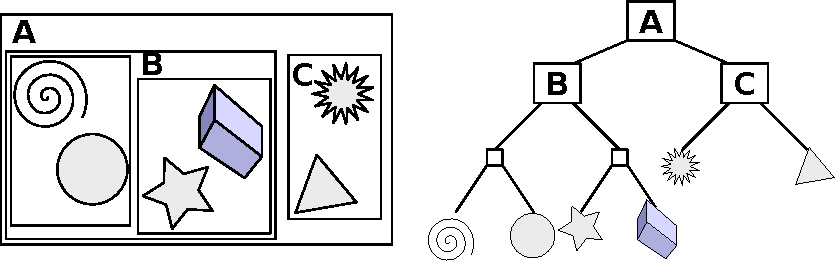
\includegraphics[width=0.8\textwidth]{bvh_example.pdf}
    \caption[Οπτικοποίηση μιας Ιεραρχίας Οριοθετικών Όγκων]{
        Παράδειγμα μιας Ιεραρχίας Οριοθετικών Όγκων στις δύο 
        διαστάσεις που χρησιμοποιεί ορθογώνια παραλληλόγραμμα 
        για οριοθετικούς όγκους.
        Αριστερά απεικονίζονται τα αντικείμενα και τα οριοθετικά 
        πλαίσια που περικλείουν τα αντικείμενα. Δεξιά απεικονίζεται 
        η ιεραρχία σε μορφή δέντρου.
        }
    \label{fig:bvh_example_2d}
\end{figure}

Γενικά, η ενθυλάκωση αντικειμένων μέσα σε οριοθετικούς όγκους επιταχύνει 
πολλές γεωμετρικές πράξεις πχ. \tl{collision detection}, \tl{ray tracing},
κλπ όπως έγινε φανερό στο \ref{sec:bounding_volumes},
παρ' όλα αυτά δε μειώνει τον αριθμό των ελέγχων που απαιτούνται.
Δηλαδή η υπολογιστική πολυπλοκότητα των αλγορίθμων παραμένει ίδια
(βλ. \ref{sec:exhaustive_search} για ένα παράδειγμα τέτοιου αλγορίθμου). 
Με την οργάνωση των αντικειμένων σε ιεραρχίες 
οριοθετικών όγκων, ωστόσο, η υπολογιστική πολυπλοκότητα (δηλαδή το πλήθος 
των ελέγχων που εκτελούνται) μπορεί να μειωθεί 
σε λογαριθμική σε σχέση με το πλήθος των αντικειμένων.
Σε μια τέτοια ιεραρχία τα αντικείμενα ενός κόμβου δε χρειάζεται 
να εξετασθούν αν το αποτέλεσμα του ελέγχου μπορεί να εξακριβωθεί 
από κάποιον πρόγονό του.
Αυτή η τεχνική ονομάζεται κλάδεμα του δέντρου (\tl{tree pruning}).

Για τη σχεδίαση ιεραρχιών οριοθετικών όγκων υπάρχουν πολλές επιλογές. 
\begin{itemize}
    \item Η \textit{επιλογή του οριοθετικού όγκου} 
    που θα χρησιμοποιείται από την ιεραρχία παίζει σημαντικό λόγο. 
    Η επιλογή καθορίζεται από μια σύμβαση μεταξύ δύο στόχων: 
    Από τη μία πλευρά, θα θέλαμε να χρησιμοποιήσουμε
    οριοθετικούς όγκους που έχουν πολύ απλό σχήμα γιατί η αποθήκευση τους 
    στη μνήμη είναι μικρή και οι διάφοροι γεωμετρικοί έλεγχοι είναι 
    γρήγοροι.
    Από την άλλη πλευρά, θα θέλαμε να έχουμε οριοθετικούς όγκους που να
    περικλείουν πολύ στενά τα αντικείμενα.
    Ο πιο κοινός τύπος οριοθετικού όγκου που χρησιμοποιείται είναι τα
    \tl{AABB}.
    
    \item Η \textit{τεχνική κατασκευής του δένδρου} αποτελεί επίσης 
    σχεδιαστική επιλογή.
    Υπάρχουν τρεις κύριες κατηγορίες αλγορίθμων κατασκευής δένδρων: 
    \begin{itemize}
        \item Οι \textit{από πάνω προς τα κάτω (\tl{top-down})}, οι 
        οποίοι λειτουργούν με διαμερισμό του συνόλου εισόδου σε δύο (ή περισσότερα)
        υποσύνολα, οριοθετώντας τα στον επιλεγμένο 
        οριοθετικό όγκο και, στη συνέχεια, επαναλαμβάνουν την ίδια 
        διαδικασία αναδρομικά έως ότου κάθε υποσύνολο να αποτελείται 
        από ένα μόνο στοιχείο (δηλαδή η διαδικασία τερματίζει 
        όταν φτάσει στα φύλλα του δέντρου).
        
        \item Οι \textit{από κάτω προς τα πάνω (\tl{bottom-up})}, οι
        οποίοι ξεκινούν με το σύνολο των στοιχείων που αποθηκεύονται 
        στα φύλλα του δέντρου και στη συνέχεια ομαδοποιούν δύο (ή περισσότερα) 
        από αυτά για να σχηματίσουν έναν νέο εσωτερικό κόμβο.
        Η διαδικασία συνεχίζεται με τον ίδιο τρόπο έως ότου όλα 
        τα στοιχεία ομαδοποιηθούν σε έναν μόνο κόμβο (τη ρίζα του δέντρου).
        Οι μέθοδοι από κάτω προς τα πάνω είναι πιο δύσκολοι στην υλοποίηση, 
        αλλά είναι πιθανό να παράγουν καλύτερης ποιότητας δέντρα γενικά.
        Ένας ευρέως διαδεδομένος τρόπος για ομαδοποίηση των δεδομένων από κάτω 
        προς τα πάνω είναι η χρήση \textit{καμπυλών πλήρωσης χώρου
        (\tl{space filling curves})} \cite{gu2013efficient} \cite{tero2012construct}. 
        Τα στοιχεία ταξινομούνται αρχικά με βάση την καμπύλη και 
        ομαδοποιούνται σύμφωνα με την ακολουθία που προκύπτει.
        
        \item Οι \textit{μέθοδοι με εισαγωγή (\tl{insertion methods})}, οι 
        οποίοι κατασκευάζουν το δέντρο εισάγοντας ένα στοιχείο τη φορά, 
        ξεκινώντας από ένα κενό δέντρο. 
        Η θέση που τοποθετείται ένα νέο στοιχείο επιλέγεται έτσι ώστε 
        το δέντρο να μεγαλώσει όσο το δυνατόν λιγότερο, σύμφωνα με κάποια 
        μετρική κόστους.
        Οι μέθοδοι με εισαγωγή θεωρούνται \tl{on-line} μέθοδοι δεδομένου ότι
        δεν απαιτούν να είναι διαθέσιμα όλα τα στοιχεία πριν από την έναρξη
        της κατασκευής και επομένως επιτρέπουν την εκτέλεση ενημερώσεων 
        (\tl{updates}) κατά το χρόνο εκτέλεσης.
        Οι άλλες δύο κατηγορίες που αναφέρθηκαν θεωρούνται \tl{off-line} 
        μέθοδοι καθώς και οι δύο απαιτούν να είναι διαθέσιμα όλα τα 
        στοιχεία πριν από την έναρξη της κατασκευής. 

        Η εισαγωγή στοιχείων στο \tl{BVH} συνήθως καταλήγει σε δέντρα με 
        χειρότερη επίδοση στα ερωτήματα σε σχέση με μια πλήρη ανακατασκευή
        από την αρχή. Οι λύσεις που προτείνονται είναι είτε η ασύγχρονη 
        ανακατασκευή του δέντρου, είτε η ανακατασκευή όταν ανιχνευθεί 
        σημαντική αλλαγή (πχ υπάρχει μεγάλη επικάλυψη κοντά στα φύλλα, 
        ή ο αριθμός των προσθαφαιρέσεων στοιχείων ξεπεράσει κάποιο 
        κατώφλι, ή άλλες πιο εκλεπτυσμένες ευρετικές μεθόδους).
    \end{itemize}
    
    \item Ο \textit{βαθμός} (αριθμός των παιδιών των κόμβων) του 
    δένδρου. 
    Ένα δέντρο χαμηλού βαθμού θα έχει μεγαλύτερο ύψος. 
    Αυτό αυξάνει τον χρόνο διάσχισης από τη ρίζα έως τα φύλλα.
    Από την άλλη πλευρά, λιγότεροι υπολογισμοί πρέπει να δαπανηθούν
    σε κάθε κόμβο που επισκέπτεται ο αλγόριθμος για να ελέγξει ποια 
    παιδιά θα επισκεφθεί και με ποια σειρά. 
    Το αντίθετο ισχύει για ένα δέντρο υψηλού βαθμού, δηλαδή αν και το δέντρο
    θα είναι μικρότερου ύψους, δαπανάται περισσότερη δουλειά σε κάθε κόμβο.
    Στην πράξη, τα δυαδικά δέντρα (βαθμός $ = 2$) είναι μακράν τα πιο κοινά. Ένας από τους κύριους λόγους είναι ότι τα δυαδικά δέντρα είναι πιο εύκολο να κατασκευαστούν.
    
    \item \textit{Η μέθοδος διάσχισης} του δένδρου για την απάντηση 
    γεωμετρικών ερωτημάτων. Όταν θα πρέπει να γίνει επίσκεψη σε 
    περισσότερα από ένα απ'ο τα παιδιά ενός κόμβου, 
    η σειρά με την οποία αυτά θα ελεγχθούν 
    δεν επηρεάζει την ορθότητα του αλγορίθμου, όμως έχει αντίκτυπο 
    στην επίδοση του.
\end{itemize}

Τέλος, αναφέρουμε κάποιες επιθυμητές ιδιότητες \cite{ericson2004real} 
μιας Ιεραρχίας Οριοθετικών Όγκων οι οποίες πρέπει να ληφθούν υπόψη 
κατά τον σχεδιασμό της για τις διάφορες εφαρμογές:
\begin{itemize}
    \item Τα στοιχεία που περιλαμβάνει οποιοδήποτε υπο-δέντρο 
    θα πρέπει να είναι κοντά το ένα στο άλλο (χωρικά). 
    Όσο πιο χαμηλά στο δέντρο, τόσο πιο κοντά θα πρέπει να 
    βρίσκονται τα αντικείμενα.
    \item Ο όγκος της επικάλυψης των αδελφικών κόμβων πρέπει να είναι ελάχιστος
    \item Κάθε κόμβος του δέντρου πρέπει να έχει τον ελάχιστο δυνατό όγκο.
    \item Το άθροισμα όλων των οριοθετικών όγκων πρέπει να είναι ελάχιστο.
    \item Θα πρέπει να δοθεί μεγαλύτερη προσοχή στους κόμβους κοντά στη 
    ρίζα του \tl{BVH}. 
    Το κλάδεμα ενός κόμβου κοντά στη ρίζα του δέντρου αφαιρεί περισσότερα αντικείμενα
    από περαιτέρω εξέταση.
    \item Το \tl{BVH} θα πρέπει να είναι όσο πιο ισορροπημένο γίνεται. 
    Η εξισορρόπηση επιτρέπει να κλαδευτεί όσο το δυνατόν μεγαλύτερο μέρος 
    του \tl{BVH} όποτε δε διασχίζεται ένα κλαδί.
\end{itemize}

\chapter{Σχετική Βιβλιογραφία}
\label{ch:related_work}
Τα ερωτήματα εγγύτητας και η ανίχνευση σύγκρουσης διερευνώνται 
εκτενώς για δεκαετίες από ερευνητές στα γραφικά υπολογιστών, στη ρομποτική,
στις προσομοίωσες, την υπολογιστική γεωμετρία και τα κινούμενα σχέδια 
υπολογιστών. 
Εκτός από την ανίχνευση σύγκρουσης και τον υπολογισμό απόστασης, υπάρχει
σημαντική βιβλιογραφία σχετική με τις Ιεραρχίες Οριοθετικών Όγκων 
(\tl{BVH}) και τις διάφορες εφαρμογές τους. 
Σε αυτό το κεφάλαιο κάνουμε αναφορά σε άρθρα της βιβλιογραφίας 
που μελετούν το ίδιο ή παρόμοιο πρόβλημα με το δικό μας
και επισημαίνουμε τις τεχνικές που χρησιμοποιούνται 
και στη δική μας μεθοδολογία.

\section{Υπολογισμός Αποστάσεων προς Αντικείμενα}

\subsection{Κοντινότερος Κόμβος Πλέγματος από Σημείο}
\label{sec:nearest_node}
Αρχικά μελετάμε το παρακάτω πρόβλημα: \textit{"Δοθέντος ενός 
πλέγματος και ενός σημείου (\tl{query-point}), ζητείται να βρεθεί 
ο κοντινότερος προς το σημείο \textbf{κόμβος} του πλέγματος"}.
Το πρόβλημα αυτό ανάγεται στο κλασικό πρόβλημα εύρεσης των \textit{$k$ 
κοντινότερων γειτόνων} από ένα σύνολο σημείων (\tl{$k$NN}, όπου $k=1$). 

Για το πρόβλημα αυτό έχουν προταθεί διάφορες λύσεις. Για παράδειγμα 
η χρήση διαγραμμάτων \tl{Voronoi} στην περίπτωση δεδομένων 
με μικρό αριθμό διαστάσεων \cite{aurenhammer1991voronoi}.
Οι σημαντικότερες όμως συνεισφορές για το συγκεκριμένο πρόβλημα είναι 
αυτές του \cite{bentley1975multidimensional} με την εισαγωγή του 
\textit{\tl{kD-Tree}}, και του \cite{yianilos1993data} με την 
εισαγωγή του \textit{\tl{VP-Tree}} (βλ. για παράδειγμα το
\cite{simon1996fast} όπου γίνεται χρήση του \textit{\tl{kD-Tree}} για τον 
υπολογισμό του κοντινότερου κόμβου ενός τριγωνικού πλέγματος 
από σημείο).

Τα δύο παραπάνω δυαδικά δέντρα αναζήτησης απαιτούν $\bigO(n*logn)$
χρόνο προεπεξεργασίας των δεδομένων (για την κατασκευή τους
από το σύνολο των $n$ σημείων του τρισδιάστατου χώρου) και 
έπειτα $\bigO(logn)$ για την απάντηση ερωτημάτων κοντινότερου 
γείτονα, στη μέση περίπτωση. 
Στο ίδιο πλαίσιο εργασίας αναπτύσσεται ο πρώτος εκ των δύο αλγορίθμων που 
προτείνουμε, για το δικό μας πρόβλημα, όπου κατασκευάζουμε μια δομή 
δεδομένων και στη συνέχεια κάνουμε ερωτήματα κοντινότερου γείτονα 
για να υπολογίσουμε την απόσταση.

Πιο συγκεκριμένα, για την κατασκευή του \tl{\textit{kD-Tree}} το σύνολο 
των σημείων ενός κόμβου διχοτομείται σε δύο υποσύνολα που αποτελούν 
τα δύο παιδιά του κόμβου. Η διαδικασία αυτή επαναλαμβάνεται αναδρομικά:
\begin{itemize}
    \item Η διχοτόμηση γίνεται με βάση κάποιον άξονα ο οποίος εναλλάσσεται κυκλικά 
    (\tl{round-robin}) για τα διαδοχικά επίπεδα του δέντρου.
    Για παράδειγμα, στις τρεις διαστάσεις, ο διαχωρισμός γίνεται πρώτα με 
    βάση τον άξονα $x$, έπειτα με βάση τον άξονα $y$, έπειτα με τον $z$, 
    ξανά με βάση τον $x$ και ούτω καθεξής.
    \item Το κριτήριο για τον διαχωρισμό του συνόλου των σημείων $V$, ενός κόμβου, 
    σε δύο υποσύνολα $L$, $R$ είναι το εξής: Χωρίς βλάβη της γενικότητας 
    θεωρούμε πως ο άξονας διαχωρισμού είναι ο $x$. Αν $m$ είναι η διάμεσος 
    των $x$-συντεταγμένων των σημείων, τότε $L = \{p \in V \mid p_x \leq m \}$ 
    και $R = \{p \in V \mid p_x >= m \}$. 
    Τα σύνολα $L$, $R$ επιλέγονται ώστε να έχουν το ίδιο πλήθος στοιχείων 
    ή να διαφέρουν κατά ένα.
    Όμοια προκύπτει το κριτήριο και για τους άλλους άξονες.
    Η διάμεσος $m$ είναι πληροφορία που αποθηκεύεται για κάθε κόμβο του δέντρου
    και χρησιμοποιείται στα ερωτήματα εύρεσης του κοντινότερου γείτονα.
\end{itemize}

Έτσι προκύπτει ένα σχεδόν πλήρες, ισορροπημένο, δυαδικό δέντρο.
Οι ιδέες 1) της διχοτόμησης του συνόλου των δεδομένων με κυκλική εναλλαγή 
του άξονα διαχωρισμού και 2) η χρήση της διαμέσου των αντίστοιχων 
συντεταγμένων για τον διαχωρισμό  
χρησιμοποιούνται \textit{αυτούσιες} και στη δική μας μεθοδολογία 
για την κατασκευή μιας Ιεραρχίας Οριοθετικών Όγκων. 
Η διαφορά είναι πως χειριζόμαστε χωρικά δεδομένα, και όχι σημεία,
επομένως επιλέγεται ένα \textit{αντιπροσωπευτικό σημείο} για κάθε 
χωρικό αντικείμενο και εφαρμόζεται η ίδια μέθοδος κατασκευής της 
ιεραρχίας. 

\begin{wrapfigure}{l}{0.3\textwidth}
    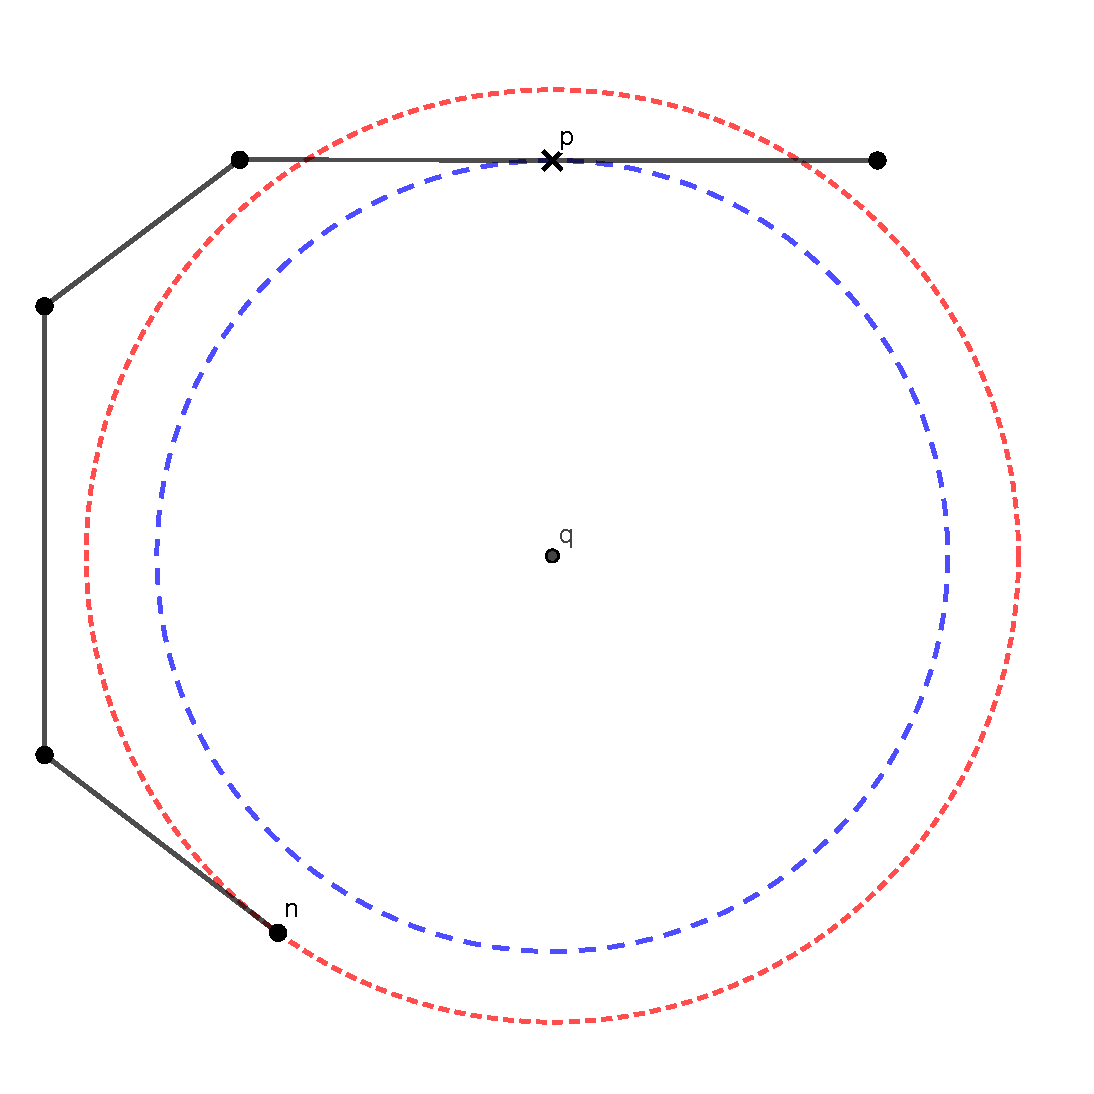
\includegraphics[width=0.29\textwidth]{nearest_node.pdf}
    \caption[Εύρεση Κοντινότερου Κόμβου από Σημείο]{
        Παράδειγμα όπου ο κοντινότερος \textit{κόμβος} $n$ ενός πλέγματος 
        διαφέρει από το κοντινότερο \textit{σημείο} $p$, δοθέντος 
        του \tl{query-point} $q$.}
    \label{fig:nearest_node}
\end{wrapfigure}

Για την κατασκευή του \tl{\textit{VP-Tree}}, ξανά, το σύνολο των σημείων 
ενός κόμβου διχοτομείται σε δύο υποσύνολα αναδρομικά:
\begin{itemize}
    \item Αρχικά, επιλέγεται ένα τυχαίο σημείο από το σύνολο $V$ των σημείων 
    του κόμβου. Το σημείο αυτό ονομάζεται \textit{\tl{vantage-point (vp)}} 
    και αποτελεί πληροφορία που αποθηκεύεται στον κόμβο.
    \item Έπειτα υπολογίζονται οι αποστάσεις όλων των υπολοίπων σημείων 
    προς το \tl{vp} και η διάμεσος $m$, που επίσης αποθηκεύεται στον κόμβο.
    \item Αν $m$ είναι η διάμεσος των αποστάσεων που υπολογίστηκαν 
    τότε το σύνολο του αριστερού παιδιού είναι το 
    $L = \{p \in V \mid distance(p,vp) \leq m \}$
    και του δεξιού παιδιού 
    $R = \{p \in V \mid distance(p,vp) \geq m \}$
\end{itemize} 

Ο τυπικός τρόπος για την απάντηση ερωτημάτων κοντινότερου κόμβου 
είναι, αρχικά, ο υπολογισμός μιας εκτίμησης αυτού διασχίζοντας το δέντρο 
από τη ρίζα έως κάποιο φύλλο. 
Το φύλλο αποτελεί την πρώτη εκτίμηση κοντινότερου κόμβου, ενώ η επιλογή του 
μονοπατιού από τη ρίζα μέχρι το φύλλο αποτελεί σχεδιαστική επιλογή και 
χρησιμοποιούνται ευρετικοί μέθοδοι (\tl{heuristics}).
Έπειτα μια σφαίρα εκτείνεται από το \tl{query-point} έως το φύλλο 
και, με τη βοήθεια του δέντρου, από τα υπόλοιπα σημεία ελέγχονται μόνο 
αυτά που βρίσκονται εντός της σφαίρας. 
Η ακτίνα της σφαίρας μικραίνει όσο ανακαλύπτονται όλο και κοντινότεροι 
κόμβοι.
Αυτή η διαδικασία λέγεται \textit{κλάδεμα (\tl{pruning})} του δέντρου,
και μειώνει τον χώρο αναζήτησης με το να απορρίπτει περιοχές που δεν 
μπορούν να περιέχουν τον κοντινότερο γείτονα. 
Με αυτόν τον τρόπο, ο αριθμός των αναμενόμενων συγκρίσεων 
είναι της τάξης $\bigO(logn)$ για τη μέση περίπτωση. 
Με ίδιο μοτίβο λογικής σχεδιάζεται και η διαδικασία αναζήτησης 
κοντινότερου γείτονα για χωρικά δεδομένα που προτείνουμε. 

Το παραπάνω πρόβλημα δεν πρέπει να συγχέεται με το πρόβλημα εύρεσης 
του κοντινότερου \textit{σημείου} ενός πολυγωνικού πλέγματος από 
κάποιο \tl{query-point}. Γενικά ο κοντινότερος \textit{κόμβος} και 
το κοντινότερο \textit{σημείο} ενός πλέγματος μπορούν να απέχουν 
πολύ μεταξύ τους όπως φαίνεται στο Σχήμα \ref{fig:nearest_node}:
Η πολυγωνική γραμμή αντιπροσωπεύει το σύνορο ενός υποθετικού πλέγματος 
στις δύο διαστάσεις και η ελάχιστη απόσταση του πλέγματος από το σημείο 
$q$ (ακτίνα του κόκκινου κύκλου) διαφέρει από την 
απόσταση του κοντινότερου κόμβου (ακτίνα του μπλε κύκλου).


% να πω για linear programming 
% These include Dobkin-
% Kirkpatrick hierarchies [DK82], linear programming [Sei90] and algorithms for intersecting
% convex p olytop es [Cha89 ] 
% και γενικά ό,τι αναφέρεται στο paper του GJK.

\subsection{Απόσταση Σημείου από Πολυγωνικό Πλέγμα}
Η περιγραφή του προβλήματος είναι η ακόλουθη: 
\textit{"Δοθέντος ενός πλέγματος και ενός σημείου του χώρου \tl{(query-point)},
ζητείται να βρεθεί το κοντινότερο \textbf{σημείο} που ανήκει 
στο πλέγμα"}.
Τα δύο παραπάνω σημεία ορίζουν την Ευκλείδεια απόσταση πλέγματος και σημείου, 
η οποία ονομάζεται και απόσταση διαχωρισμού (πλέγματος και σημείου).

Αν και το πρόβλημα υπολογισμού της Ευκλείδειας απόστασης δύο αντικειμένων 
στο χώρο αποτελεί γενίκευση του παραπάνω προβλήματος, στο 
\cite{guezlec2001meshsweeper} υποστηρίζεται ότι αξίζει να μελετηθεί 
ξεχωριστά γιατί μπορούν να αναπτυχθούν πιο αποδοτικοί αλγόριθμοι.
Στην προαναφερθείσα δημοσίευση, χρησιμοποιείται μια ιεραρχία οριοθετικών 
όγκων πολλαπλών αναλύσεων που δημιουργείται από γεωμετρική απλοποίηση 
του πλέγματος. 
Καθώς η ανάλυση του πλέγματος βελτιώνεται, ολοένα και πιο ακριβής γίνεται 
η εκτίμηση του κοντινότερου σημείου, ενώ ταυτόχρονα ο αλγόριθμος σε κάθε βήμα 
μπορεί να παρέχει τα άνω και κάτω φράγματα του σφάλματος της εκτίμησης.
Οι οριοθετικοί όγκοι που χρησιμοποιούνται στην ιεραρχία είναι τρίγωνα 
που σαρώνονται από μια σφαίρα (\tl{triangles swept by sphere}) και 
αποτελούν γενίκευση της οριοθετικής κάψουλας. 
  
\subsection{Απόσταση Δύο Αντικειμένων}
% Ο ορισμός του προβλήματος υπολογισμού της Ευκλείδειας απόστασης δύο αντικειμένων 
% έχει δοθεί στο \ref{sec:problem_description}.

% Απόσταση Δύο Πολυγωνικών Πλεγμάτων
% Απόσταση Αντικειμένων που Περιγράφονται από \tl{NURBS}
\section{Οργάνωση Χωρικών Δεδομένων σε Ιεραρχίες}
Η ιεραρχική οργάνωση των αντικειμένων του χώρου σε δενδρικές 
δομές δεδομένων αποτελεί κοινή μεθοδολογία για πολλά προβλήματα 
της Υπολογιστικής Γεωμετρίας. 
Τέτοιες δομές χρησιμοποιούνται σε διάφορες εφαρμογές για να 
επιταχύνουν τη διαδικασία επίλυσης του εκάστοτε προβλήματος, 
όπως ακριβώς συμβαίνει και στη μεθοδολογία που προτείνουμε. 
Για τον λόγο αυτό πολλές φορές αναφέρονται και ως \textit{δομές 
δεδομένων επιτάχυνσης (\tl{acceleration data structures})}.

Χαρακτηριστικά παραδείγματα αποτελούν:
\begin{itemize}
    \item Οι δομές \tl{\textit{VP-Tree}, \textit{kD-Tree}} που 
    περιγράφονται στο \ref{sec:nearest_node} και χρησιμοποιούνται 
    για το πρόβλημα εύρεσης των $k$ κοντινότερων γειτόνων (\tl{\textit{kNN}}). 

    \item Το \tl{\textit{R-Tree}} που περιγράφεται στο \cite{guttman1984r}, 
    και χρησιμοποιείται ως ευρετήριο σε βάσεις δεδομένων που αποθηκεύουν χωρικά 
    δεδομένα/αντικείμενα.
    Το \tl{R-Tree} χρησιμοποιεί \textit{ελάχιστα οριοθετικά παραλληλόγραμμα (\tl{MBR})}
    για την οργάνωση των χωρικών αντικειμένων, από τα φύλλα έως τη ρίζα και ανήκει 
    στην οικογένεια των Ιεραρχιών Οριοθετικών Όγκων (\tl{BVH}).

    Υποστηρίζει εισαγωγή, διαγραφή και ενημέρωση δεδομένων καθώς επίσης 
    και ερωτήματα εύρεσης των αντικειμένων που βρίσκονται εντός μιας δοθείσας περιοχής. 
    Γενικά, το \tl{R-Tree} δεν είναι δυαδικό δέντρο και ο τρόπος διάσχισης του 
    δεν είναι τετριμμένος.
    Στο \cite{roussopoulos1995nearest} περιγράφεται ένας αλγόριθμος 
    εύρεσης των $k$ κοντινότερων αντικειμένων από κάποιο σημείο $p$, για το \tl{R-Tree}.
    Στον αλγόριθμο αυτόν εισάγωνται οι μετρικές απόστασης \textit{\tl{MINDIST}}
    και \textit{\tl{MINMAXDIST}} βάση των οποίων ορίζεται η σειρά της αναζήτησης 
    με κάποια προτεραιότητα.
    Οι μετρικές αποτελούν το κάτω και άνω φράγμα, αντίστοιχα, της απόστασης του 
    αντικειμένου από το σημείο $p$.

    \item Το \tl{\textit{BSP-Tree}}, που περιγράφεται στο \cite{fuchs1980visible},
    χρησιμοποιείται για την απόδοση γραφικών καθώς μπορεί να δώσει χωρικές πληροφορίες 
    για τα αντικείμενα μιας σκηνής. 
    Συνήθως τα αντικείμενα είναι πολύγωνα στον τρισδιάστατο χώρο.
    Η δομή του επιτρέπει την εύκολη διάσχιση των αντικειμένων μιας σκηνής από πίσω προς 
    τα εμπρός για δοσμένη θέση θέασης.

    Συγκεκριμένα, η κατασκευή του γίνεται μια μόνο φορά για κάποια στατική σκηνή 
    και το ίδιο δέντρο μπορεί να χρησιμοποιηθεί για οποιαδήποτε γωνία θέασης.
    Για την κατασκευή του, ο χώρος διαχωρίζεται αναδρομικά 
    σε δύο ημι-χώρους (\tl{half-spaces}) με βάση κάποιο επίπεδο.
    Τα αντικείμενα (ολόκληρα ή κάποιο μέρος τους) τοποθετούνται στο αριστερό ή δεξί
    παιδί ανάλογα με τον ημι-χώρο στον οποίο ανήκουν.
    Παρόλο που αποθηκεύει χωρικά δεδομένα (και όχι σημεία), το \tl{BSP-Tree} 
    θεωρείται γενίκευση του \tl{kD-Tree} διότι τα επίπεδα που χωρίζουν 
    τον χώρο μπορεί να έχουν οποιονδήποτε προσανατολισμό σε αντίθεση 
    με τα ευθυγραμμισμένα με τους άξονες επίπεδα του \tl{kD-Tree}.

    \item Το \tl{\textit{OBBTree}}, που περιγράφεται στο \cite{gottschalk1996obbtree}
    ανήκει, επίσης, στην οικογένεια των Ιεραρχιών Οριοθετικών Όγκων και χρησιμοποιεί 
    \textit{προσανατολισμένα οριοθετικά πλαίσια (\tl{OBB})}. 
    Χρησιμοποιείται για την ανίχνευση σύγκρουσης αντικειμένων που αναπαρίστανται 
    από πολυγωνικά πλέγματα. 
    Για την κατασκευή του δέντρου είναι απαραίτητα: 
    \begin{enumerate}
        \item Μια διαδικασία που για δοσμένο σύνολο πολυγώνων υπολογίζει 
        κάποιο \tl{OBB} με παρόμοιες διαστάσεις και προσανατολισμό
        ώστε να περικλείει τα πολύγωνα.
        \item Ένας τρόπος οργάνωσης των \tl{OBB} σε ιεραρχία.
    \end{enumerate}
    Στην παραπάνω δημοσίευση, για τον υπολογισμό του \tl{OBB} αρχικά κάθε πολύγωνο
    διασπάται σε τρίγωνα και έπειτα χρησιμοποιούνται στατιστικά
    πρώτης και δεύτερης τάξης που περιγράφουν τις συντεταγμένες των κόμβων
    (μέσος όρος και πίνακας συνδιακύμανσης).
    Έτσι υπολογίζεται ένα ορθοκανονικό σύστημα συντεταγμένων για τον προσανατολισμό 
    του \tl{OBB} και το μέγεθος του ορίζεται από τα ακραία σημεία κατά μήκος κάθε άξονα.
    
    Για την οργάνωση των \tl{OBB} σε ιεραρχία προτείνεται μια μέθοδος από 
    πάνω προς τα κάτω: ο μεγαλύτερος άξονας του \tl{OBB}
    χωρίζεται με βάση ένα επίπεδο κάθετο προς τον άξονα και 
    τα πολύγωνα διαχωρίζονται ανάλογα τη μεριά του επιπέδου που αντιστοιχίζεται 
    το κέντρο τους.
    Η συντεταγμένη του επιπέδου διαχωρισμού κατά μήκος αυτού του άξονα
    επιλέγεται να είναι η μέση τιμή των συντεταγμένων των κόμβων.
    Αντί για τη μέση τιμή μπορεί να χρησιμοποιηθεί η διάμεσος, οπότε 
    το δέντρο που θα προκύψει είναι ισορροπημένο. 
    Ο χρόνος κατασκευής του δέντρου με τον παραπάνω αλγόριθμο είναι της 
    τάξης $\bigO(nlogn)$, για ένα σετ με $n$ τρίγωνα. 
    
    Έχοντας τα \tl{OBBTree} για δύο αντικείμενα ο αλγόριθμος 
    για τον έλεγχο σύγκρουσης, τυπικά, ξοδεύει τον περισσότερο 
    χρόνο ελέγχοντας ζευγάρια από \tl{OBB} για επικάλυψη.   
    Για τον έλεγχο επικάλυψης δύο \tl{OBB} σχεδιάζεται ειδική ρουτίνα
    όπου γίνεται χρήση του \textit{θεωρήματος του διαχωριστικού άξονα 
    (\tl{separating axis theorem - \textbf{SAT}})} 
    \cite{gottschalk1996separating}.

    \item Το \tl{\textit{Octree}}, που περιγράφεται στο \cite{meagher1982geometric}
    χρησιμοποιείται σε πολλές εφαρμογές για απόδοση γραφικών, ανίχνευση σύγκρουσης, 
    ανίχνευση ακτίνων, ως χωρικό ευρετήριο, ως γεννήτρια πλεγμάτων κ.α. 
    Ένας κόμβος του δέντρου μπορεί να έχει έως και οκτώ παιδιά που κάθε ένα
    αντιπροσωπεύει ένα ογδοημόριο του τρισδιάστατου χώρου που καταλαμβάνει ο 
    πατρικός κόμβος. 
    Τα ογδοημόρια είναι οριοθετικά πλαίσια ευθυγραμμισμένα με τους άξονες.

    Συνήθως για την κατασκευή του, αρχικά ορίζεται το ελάχιστο μέγεθος που μπορεί να 
    έχει ένα ογδοημόριο και ο χώρος που καταλαμβάνει η ρίζα του δέντρου. 
    Έπειτα κάθε κόμβος του  δέντρου 
    διαιρείται σε ογδοημόρια μέχρι είτε να μην περιέχεται κανένα αντικείμενο 
    εντός του ογδοημορίου, είτε το ογδοημόριο να πάρει το ελάχιστο δυνατό μέγεθος.
    Οι κόμβοι του δέντρου που δεν περιέχουν τίποτα στο εσωτερικό τους μπορούν να αγνοηθούν.
    Έτσι, οποιοδήποτε τρισδιάστατο αντικείμενο μπορεί να αναπαρασταθεί με οσοδήποτε 
    μεγάλη ανάλυση (\tl{resolution}).

    Στην παραπάνω δημοσίευση περιγράφονται επίσης αλγόριθμοι για τις διάφορες 
    πράξεις μεταξύ αντικειμένων που αναπαρίστανται από \tl{Octrees}.
    Τέτοιες είναι οι πράξεις της ένωσης, τομής, διαφοράς, οι γεωμετρικές πράξεις 
    μεταφοράς, περιστροφής, κλιμάκωσης και η ανίχνευση σύγκρουσης και απόδοσης γραφικών 
    από οποιαδήποτε γωνία θέασης. 
\end{itemize}

Πολλές από τις τεχνικές που αναφέρονται παραπάνω ακολουθούνται και 
στη δική μας μεθοδολογία.
Παραδείγματα αποτελούν η χρήση οριοθετικών όγκων και η αναδρομική οργάνωση 
των αντικειμένων σε μια ιεραρχία, η μοντελοποίηση του προβλήματος 
ως πρόβλημα κοντινότερων γειτόνων για χωρικά δεδομένα και ο 
ορισμός της σειράς επίσκεψης των κόμβων της ιεραρχίας, κατά την αναζήτηση, με 
βάση μια μετρική απόστασης.

Τέλος, αξίζει να σημειωθεί ότι στη βιβλιογραφία γίνεται λόγος για την 
ποιότητα των Ιεραρχιών Οριοθετικών Όγκων. 
Ορίζονται μετρικές ποιότητας που χρησιμεύουν τόσο στην αξιολόγηση όσο 
και στην κατασκευή των ιεραρχικών δομών.
Επί του παρόντος, δεν υπάρχει πρακτικός τρόπος για τον προσδιορισμό 
του βέλτιστου διαχωρισμού των αντικειμένων ενός κόμβου σε δύο υποσύνολα.
Έτσι, δεν είναι γνωστό ποια αντικείμενα πρέπει να ομαδοποιηθούν μαζί
με άλλα για να επιτευχθεί η καλύτερη δυνατή επίδοση των αλγορίθμων.
Η πιο διαδεδομένη μετρική κόστους είναι η 
\textit{\tl{SAH (Surface Area Heuristic)}} 
\cite{goldsmith1987automatic} \cite{macdonald1990heuristics}
η οποία, περιληπτικά, "επιβραβεύει" μικρούς χωρικά κόμβους με πολλά 
αντικείμενα και "τιμωρεί" μεγάλους κόμβους με λίγα τρίγωνα. 
Επίσης, στο \cite{aila2013quality} εισάγωνται οι μετρικές 
\tl{\textit{EPO (End-point Overlap)}} και 
\tl{\textit{LCV (Leaf Count Variability)}} ως συμπληρωματικές 
της \tl{SAH} για να εξηγήσουν την παρατηρούμενη επίδοση 
των δέντρων σε περιπτώσεις όπου η \tl{SAH} αδυνατεί να 
δικαιολογήσει την επίδοση κάποιων δέντρων συγκριτικά 
με άλλα.

\chapter{Μεθοδολογία}
\label{ch:methodology}

\section{Υπολογισμοί Απόστασης Στοιχειωδών Γεωμετρικών Αντικειμένων}
\subsection{Ευκλείδεια Απόσταση δύο Τριγώνων}
\subsubsection{Ευκλείδεια Απόσταση δύο Ευθυγράμμων Τμημάτων}
\subsubsection{Ευκλείδεια Απόσταση Σημείου και Τριγώνου}
\subsection{Ευκλείδεια Απόσταση δύο \tl{AABB}}

\section{Αλγόριθμοι Εξαντλητικής Αναζήτησης}

\section{Ορισμός Μετρικής Κόστους Αναζήτησης}
\label{sec:cost_metric}

\section{Σχεδιασμός μιας \tl{BVH} Δομής Δεδομένων, το \tl{spatial KD-Tree}}
\subsection{Κατασκευή του \tl{sKD-Tree}}
\subsection{Ερωτήματα Κοντινότερου Γείτονα στο \tl{sKD-Tree}}

\section{Αλγόριθμοι που χρησιμοποιούν τη δομή \tl{sKD-Tree}}

\section{Βελτιστοποίηση των Αλγορίθμων για Πραγματικά Συστήματα Υπολογιστών}
\subsection{Παραλληλοποίηση με χρήση Πολλαπλών Νημάτων \tl{(Multi-threading)}}
\subsection{Χρήση Κουβάδων στα Φύλλα του \tl{sKD-Tree (Buckets)}}
\chapter{Πειράματα και Αποτελέσματα}
\label{ch:experiments}
Η εκτέλεση όλων των πειραμάτων που παρουσιάζονται παρακάτω 
πραγματοποιήθηκε σε πόρους της Ιδρυματικής συστοιχίας του 
ΑΠΘ "Αριστοτέλης".
Το μοντέλο επεξεργαστή που χρησιμοποιήθηκε για τα πειράματα 
είναι \tl{Intel Xeon E5-2630 v4}.
Η υλοποίηση των αλγορίθμων έγινε στη γλώσσα \tl{"Julia Version
1.7.2"}. 


\section{Κόστος Υπολογισμού Απόστασης Στοιχείων}
\label{sec:geom_tests_cost}
Για τον προσδιορισμό του κόστους $C_v$ και $C_p$
της μετρικής κόστους της ενότητας \ref{sec:cost_metric}
θεωρήσαμε πως το κόστος υπολογισμού της τετραγωνική απόστασης
δύο σημείων είναι μονάδα.
Όλα τα υπόλοιπα κόστη, λοιπόν, υπολογίζονται σε σχέση με το 
κόστος σημείο-σημείο. 
Μετρήσαμε τον χρόνο υπολογισμού των τετραγωνικών αποστάσεων 
περίπου $210\times10^6$ σημείων, \tl{AABB}, ευθυγράμμων τμημάτων 
και τριγώνων και προέκυψε ο πίνακας \ref{tab:distance_rel_cost} 
με τα σχετικά κόστη. Επομένως, $C_v=23.5$, $C_p=385.7$.

\begin{table}[h]
    \centering
    \begin{tabular}{|c|c|}
        \hline 
        Υπολογισμός Απόστασης & Κόστος \\
        \hline
        Σημείο-Σημείο & $1$ \\
        \hline 
        AABB-AABB & $23.5$ \\
        \hline
        Ευθ. Τμήμα - Ευθ. Τμήμα & $129.8$ \\
        \hline
        Τρίγωνο-Τρίγωνο & $385.7$ \\
        \hline
    \end{tabular}
    \caption[]{Σχετικό κόστος υπολογισμού της απόστασης διαφόρων στοιχείων}
    \label{tab:distance_rel_cost}
\end{table}

\section{Κατασκευή Δεδομένων Ελέγχου}
Για την εκτέλεση των πειραμάτων κατασκευάσαμε διάφορα σενάρια.
Κάθε σενάριο αποτελείται από δύο αντικείμενα και για το κάθε 
αντικείμενο κατασκευάσαμε τριγωνικά πλέγματα με τρεις διαφορετικές 
αναλύσεις (διαφορετικό πλήθος τριγώνων).
Έτσι, για κάθε σενάριο εκτελούμε ερωτήματα εύρεσης της απόστασης 
των αντικειμένων για κάθε συνδυασμό ανάλυσης (σύνολο 9 μετρήσεις).
Έγινε προσπάθεια συμπερίληψης διάφορων περιπτώσεων, με αντικείμενα 
διαφόρων σχημάτων, διαστάσεων και προσανατολισμού.

Η λήψη των αντικειμένων που χρησιμοποιούνται σε αυτή την εργασία 
έγινε από το \tl{GrabCAD}\cite{GrabCAD} και το \tl{3D Content Central}
\cite{3dcontentcentral}. 
Τα αντικείμενα, αρχικά, ήταν σε μορφή \tl{\texttt{IGES}}, ενώ για τη 
δημιουργία των πλεγμάτων χρησιμοποιήθηκε το πρόγραμμα 
\tl{BETA CAE SYSTEMS - Ansa v21.0.0}.

\begin{figure}[H]
    \begin{subfigure}{0.49\textwidth}
        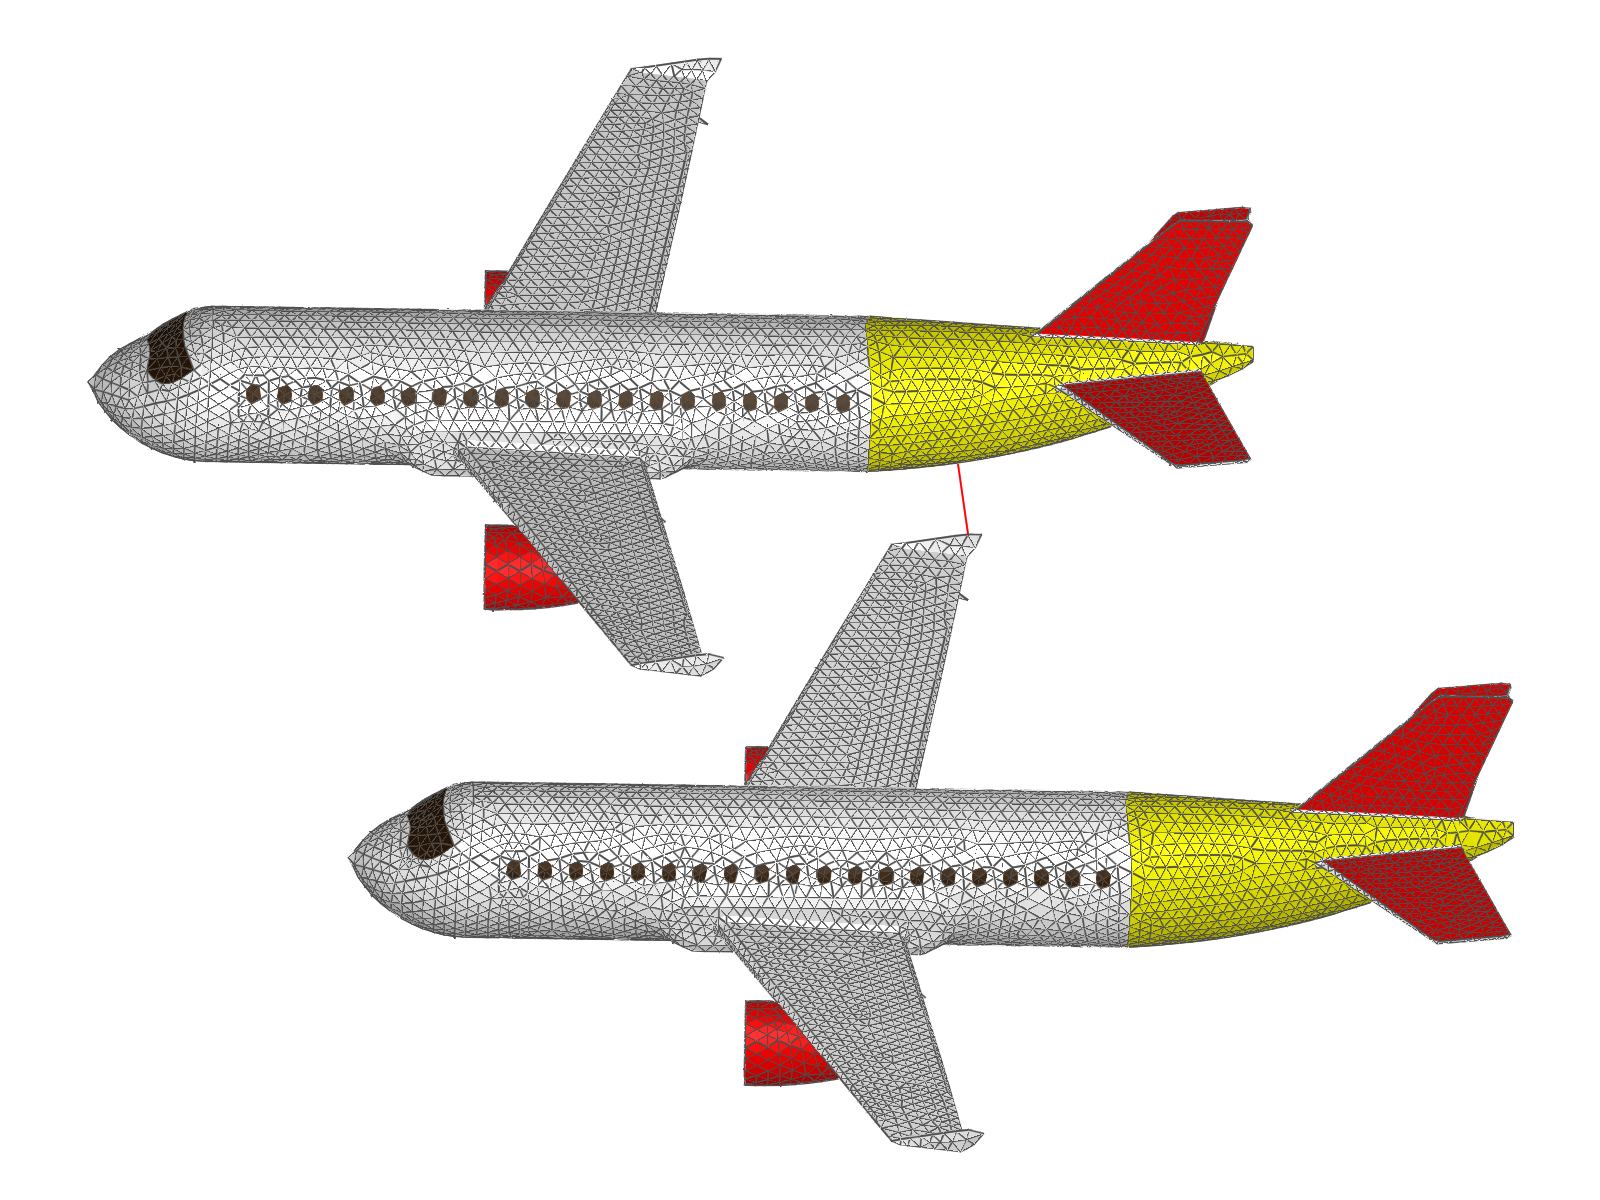
\includegraphics[width=0.9\textwidth]{testcase_scenes/airplanes_scene.png}
        \caption{Αεροπλάνα}
    \end{subfigure}
    \begin{subfigure}{0.49\textwidth}
        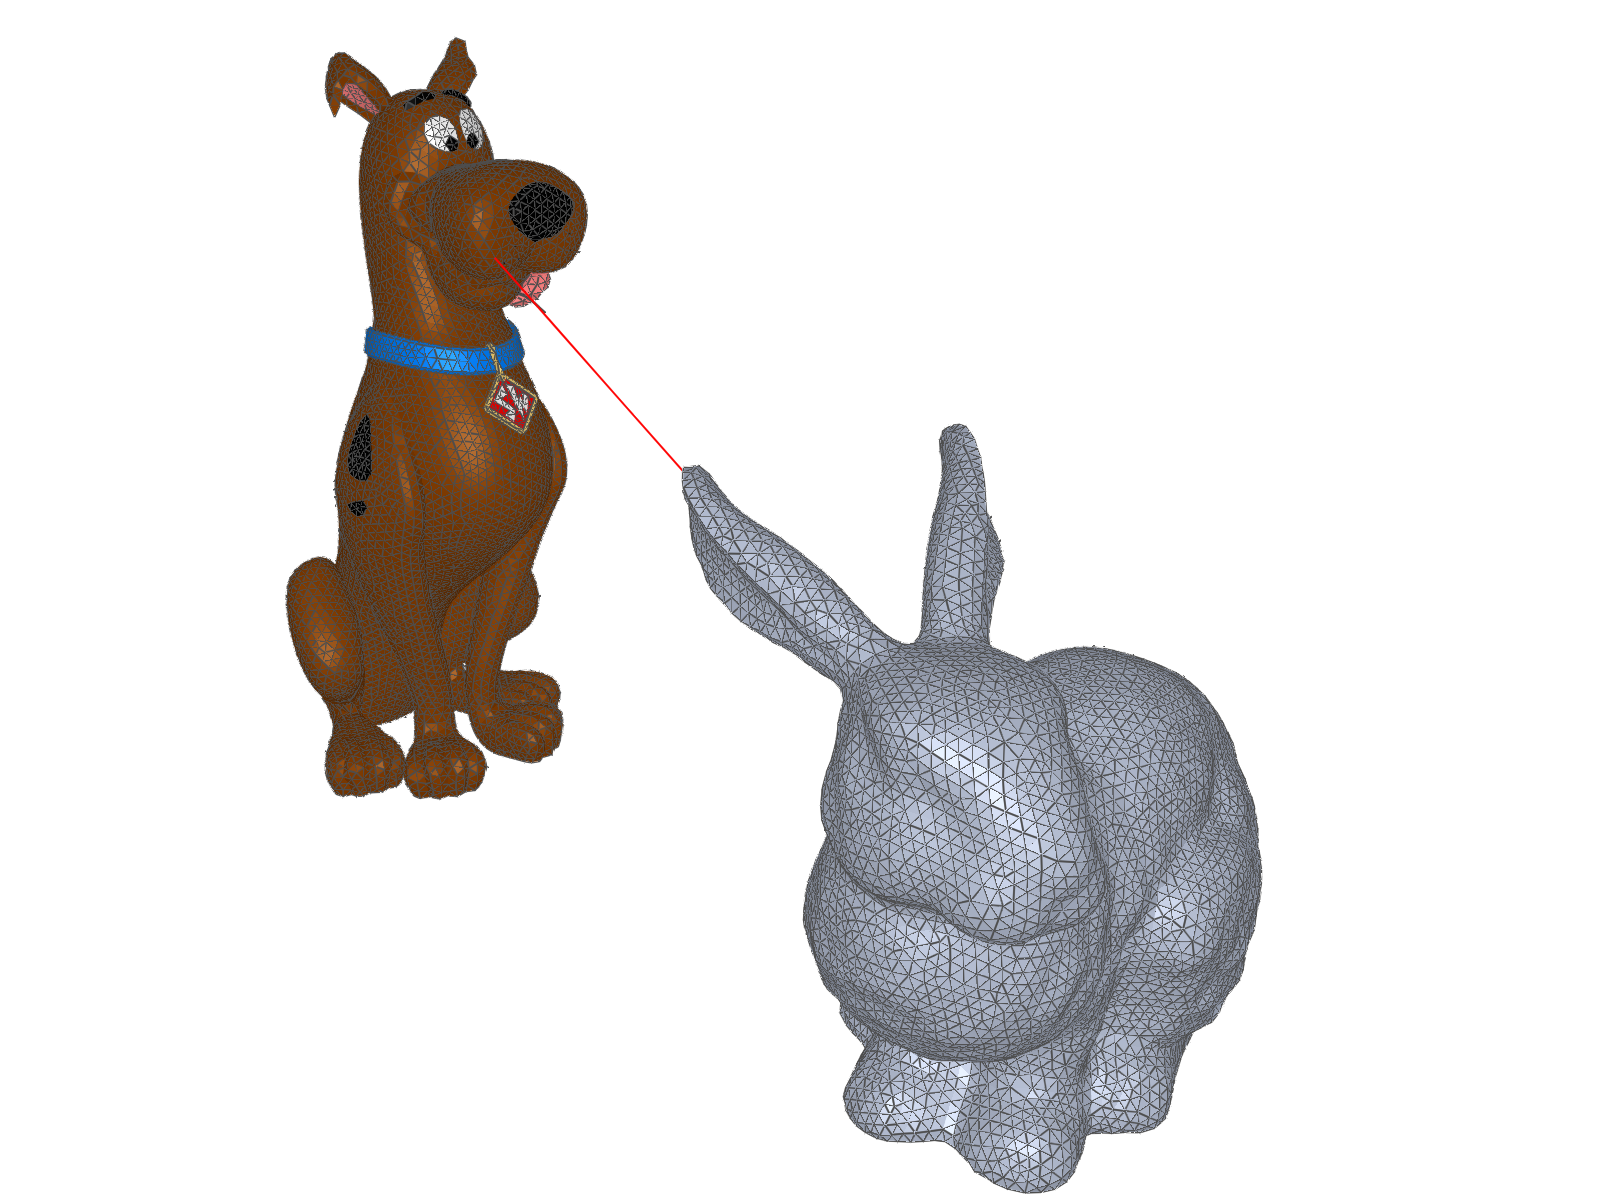
\includegraphics[width=0.9\textwidth]{testcase_scenes/scooby_w_bunny_scene.png}
        \caption{\tl{Scooby} με \tl{Stanford Bunny}}
    \end{subfigure}
    \begin{subfigure}{0.49\textwidth}
        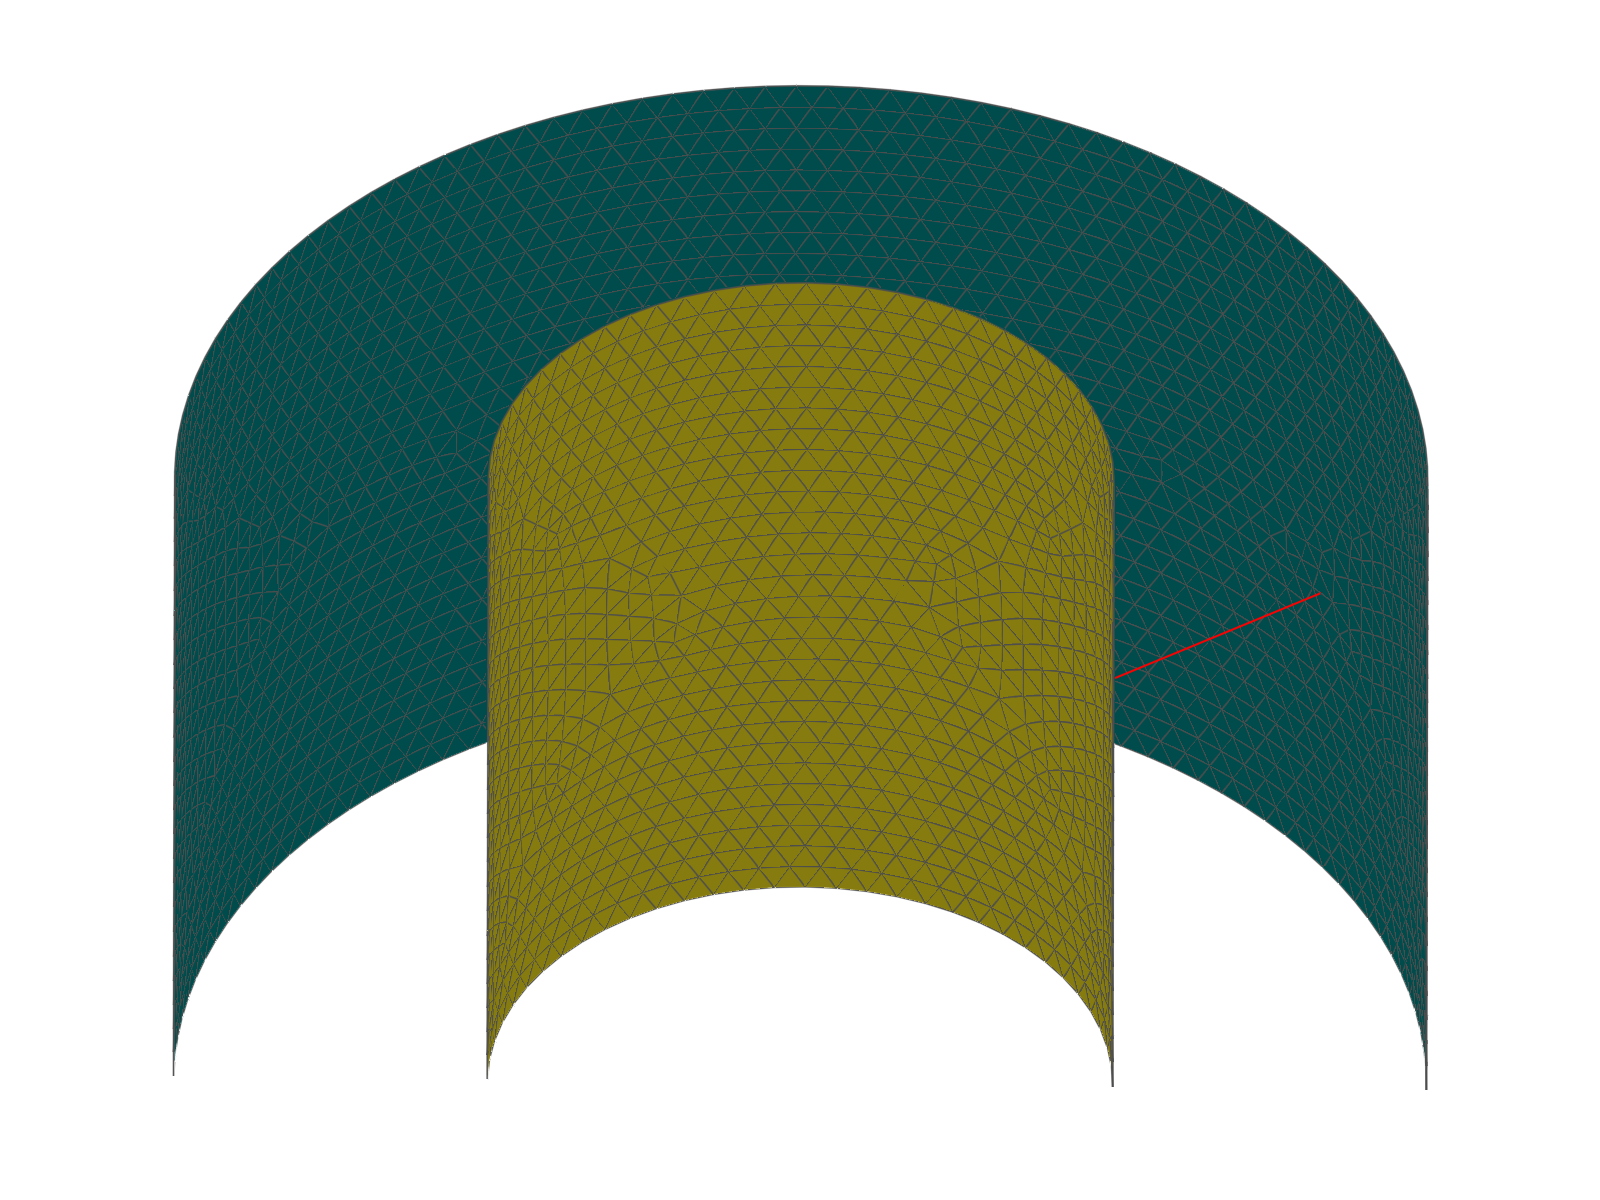
\includegraphics[width=0.9\textwidth]{testcase_scenes/cylinders_scene.png}
        \caption{Ομοαξονικοί ημι-κύλινδροι}
    \end{subfigure}
    \begin{subfigure}{0.49\textwidth}
        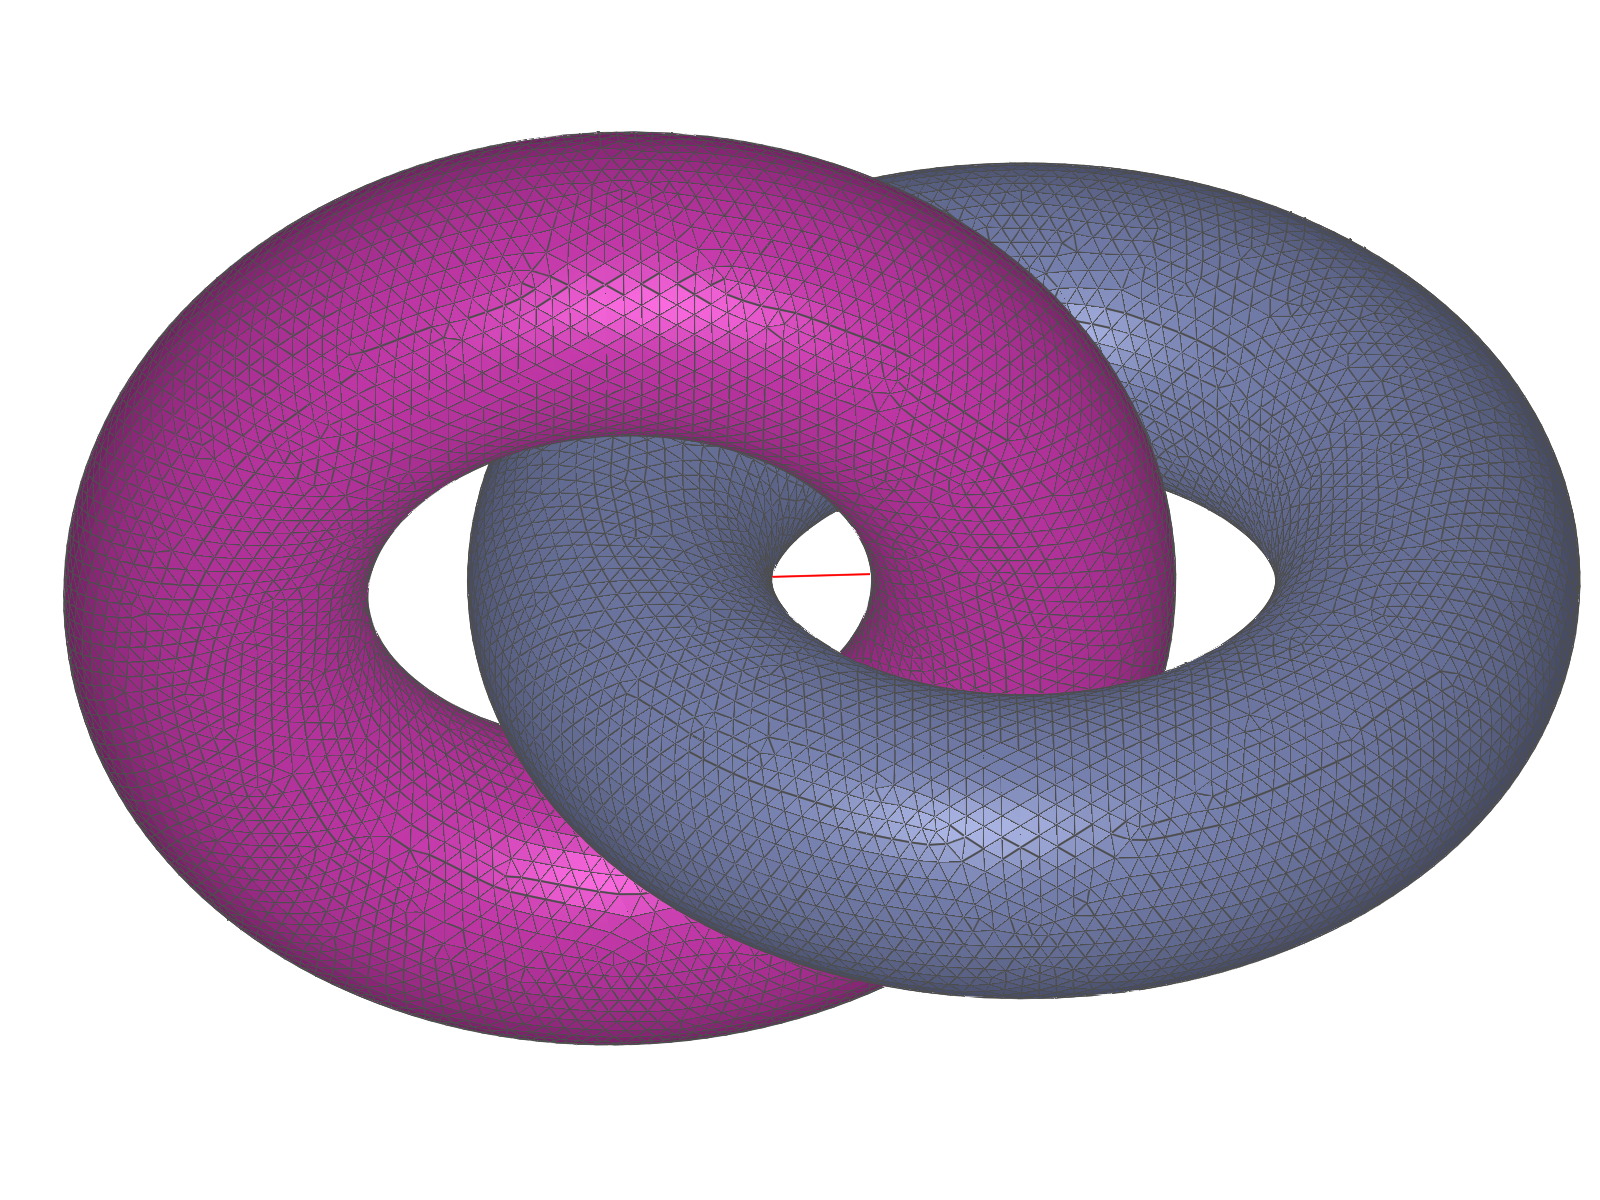
\includegraphics[width=0.9\textwidth]{testcase_scenes/chained_tori_scene.png}
        \caption{Αλυσιδωτοί Τόροι}
    \end{subfigure}
    \centering
    \begin{subfigure}{0.49\textwidth}
        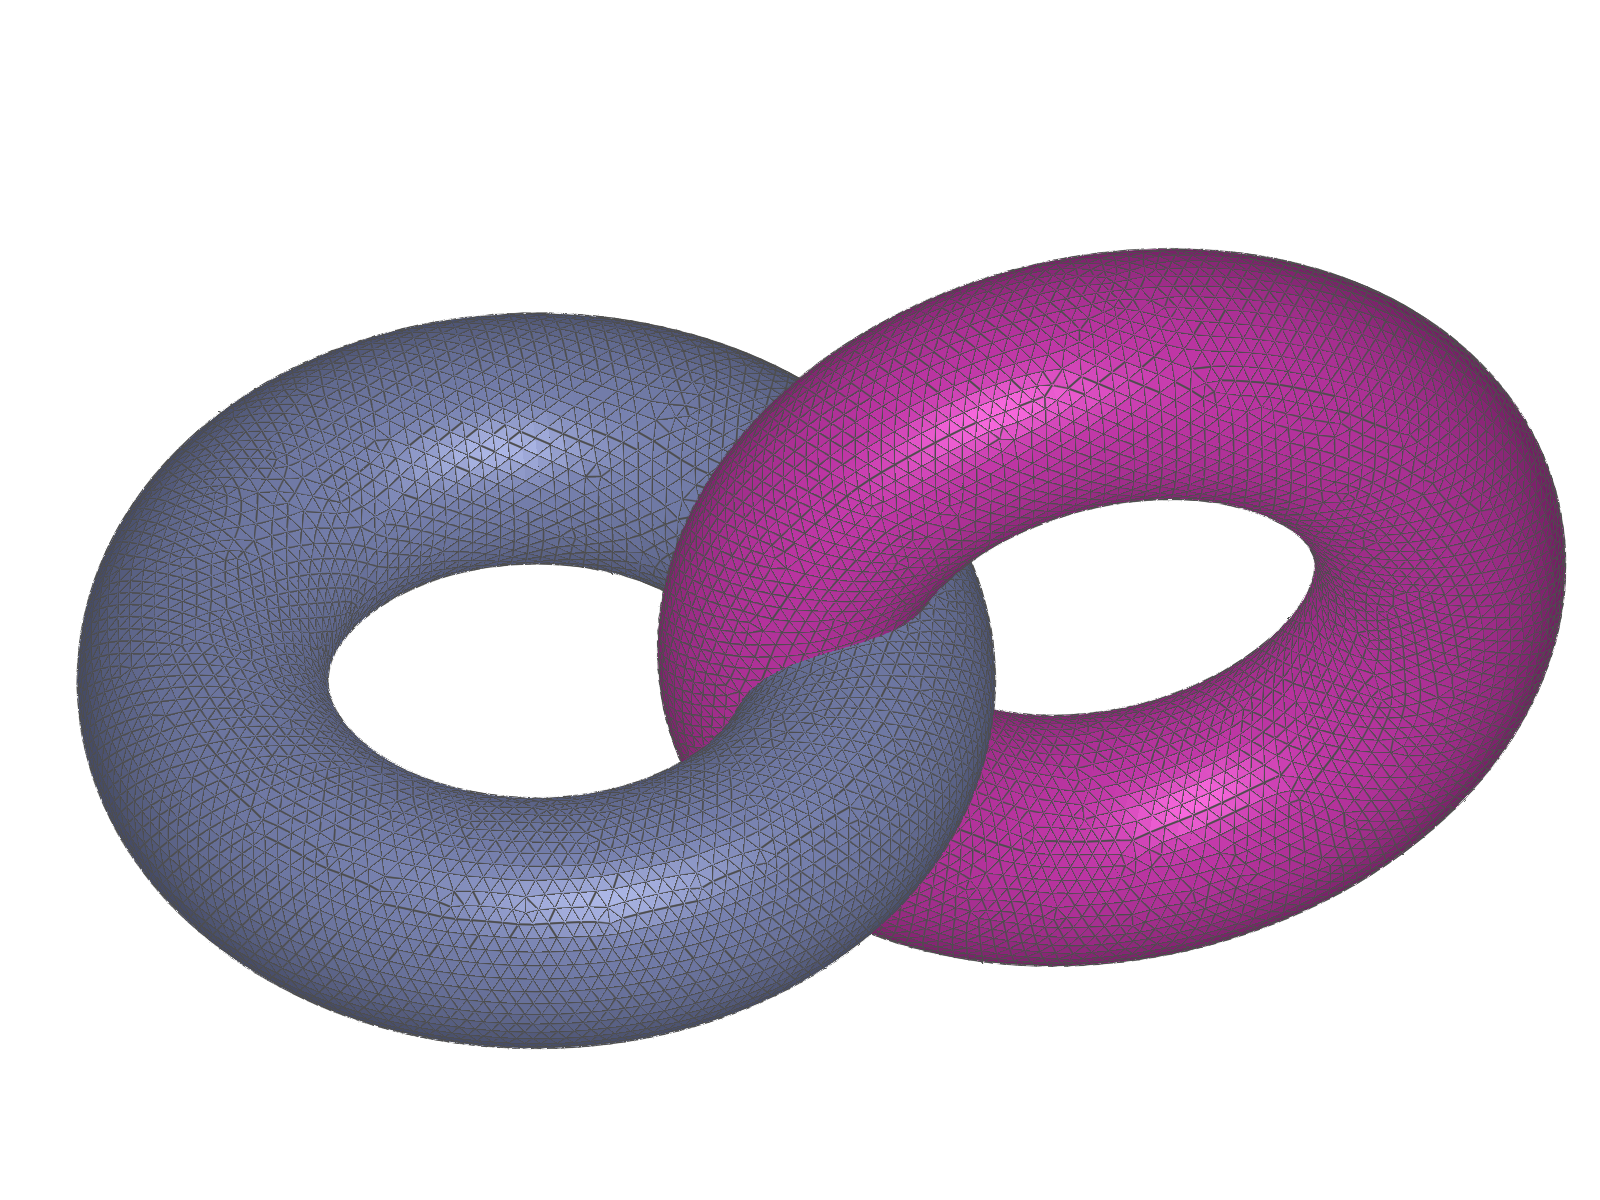
\includegraphics[width=0.9\textwidth]{testcase_scenes/colliding_tori_scene.png}
        \caption{Συγκρουόμενοι Τόροι}
    \end{subfigure}
    \caption[Οπτική αναπαράσταση των σεναρίων των πειραμάτων]{
        Οπτική αναπαράσταση των σεναρίων που χρησιμοποιήθηκαν για την 
        εκτέλεση των πειραμάτων της παρούσας εργασίας.
        Κάθε σενάριο αποτελείται από μία σκηνή με δύο αντικείμενα.  
        Το κόκκινο ευθύγραμμο τμήμα αναπαριστά την Ευκλείδεια απόσταση 
        των αντικειμένων.
    }
    \label{fig:scenarios_photos}
\end{figure}

\section{Χρόνος Κατασκευής του \tl{sKD-Tree}}
Στο σχήμα \ref{fig:build_time} παρουσιάζονται οι μετρήσεις του 
χρόνου κατασκευής του \tl{sKD-Tree} συναρτήσει του μεγέθους ενός 
τριγωνικού πλέγματος και του πλήθους των νημάτων (\tl{threads})
που χρησιμοποιήθηκαν.

\begin{figure}[h]
    \centering
    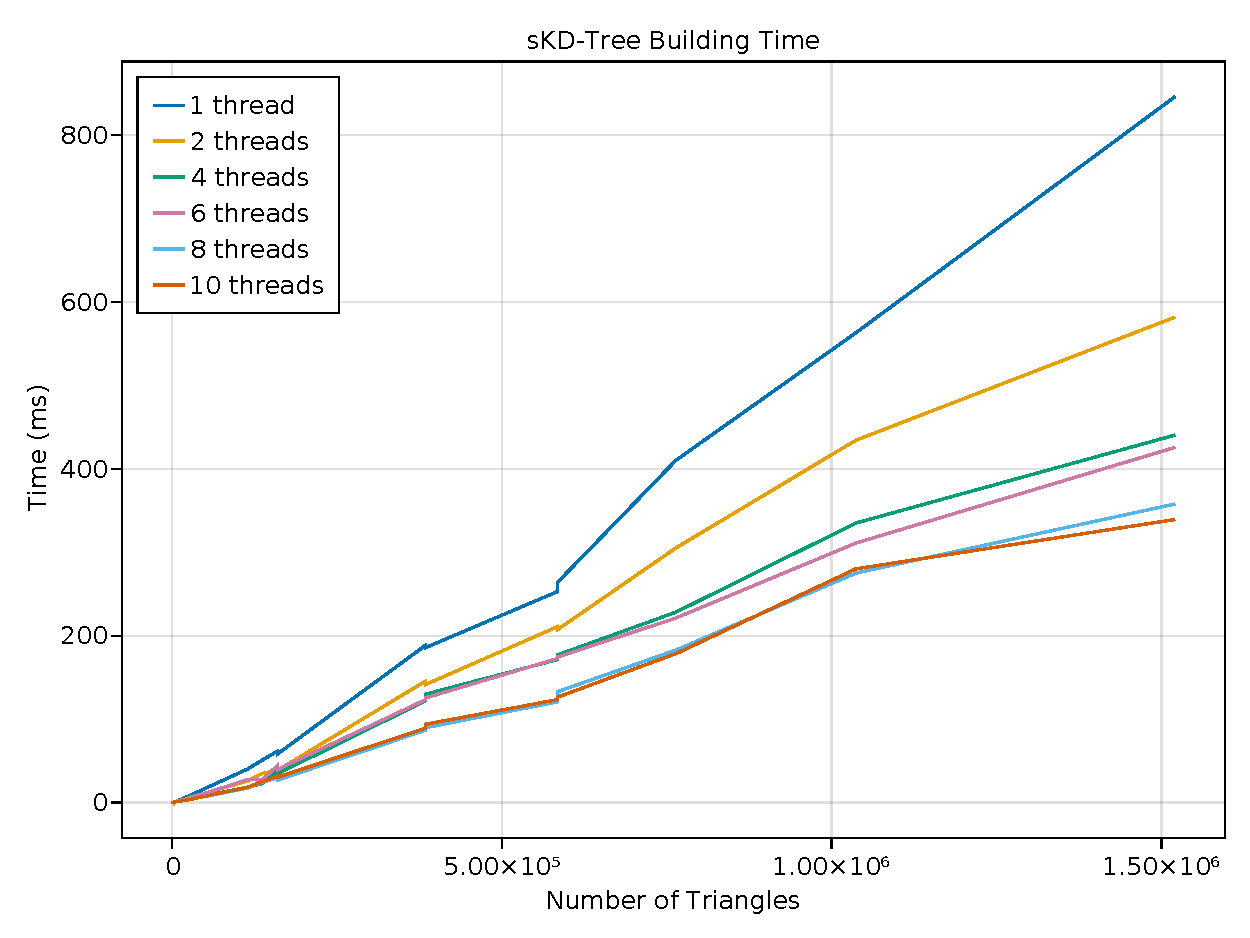
\includegraphics[width=0.6\textwidth]{build_time.pdf}
    \caption[Χρόνοι Κατασκευής του \tl{sKD-Tree}]{
        Χρόνος κατασκευής του \tl{sKD-Tree} συναρτήσει 
        του πλήθους των τριγώνων ενός πλέγματος.
    }
    \label{fig:build_time}
\end{figure}

\section{Πειράματα ανά Σενάριο}
Για κάθε ένα από τα παρακάτω σενάρια, παρουσιάζονται οι 
μετρήσεις για το κόστος αναζήτησης και το συνολικό χρόνο 
εκτέλεσης για την απάντηση ερωτημάτων απόστασης.
Στα διαγράμματα παρακάτω, γίνεται σύγκριση της επίδοσης των αλγορίθμων 
\ref{alg:queries_on_tree} και \ref{alg:search_on_two_trees}.

Το κόστος αναζήτησης υπολογίστηκε από τη μετρική κόστους 
που περιγράφεται στην ενότητα \ref{sec:cost_metric} 
μετρώντας τον αριθμό κλήσεων των ρουτινών 
\tl{\texttt{triangle\_distance()}} και \tl{\texttt{AABB\_distance()}}.
Σημειώνεται πως η καταμέτρηση των κλήσεων στις παραπάνω ρουτίνες 
πραγματοποιήθηκε για τη σειριακή εκτέλεση των αλγορίθμων, και συγκεκριμένα 
του αλγορίθμου \ref{alg:queries_on_tree}, αφού ο αλγόριθμος 
\ref{alg:search_on_two_trees} δεν είναι παράλληλος εκ κατασκευής.

Ο συνολικός χρόνος εκτέλεσης ερωτημάτων απόστασης περιλαμβάνει 
το χρόνο προεπεξεργασίας των δεδομένων και τον χρόνο αναζήτησης.
Η προεπεξεργασία των δεδομένων είναι η κατασκευή ενός ή δύο δέντρων 
ανάλογα με τον αλγόριθμο που χρησιμοποιείται.
Οι χρόνοι που παρουσιάζονται αντιστοιχούν σε πειράματα με χρήση 
ενός, τεσσάρων και οκτώ νημάτων επεξεργασίας.

\subsection{Αεροπλάνα}

\begin{figure}[H]
    \centering
    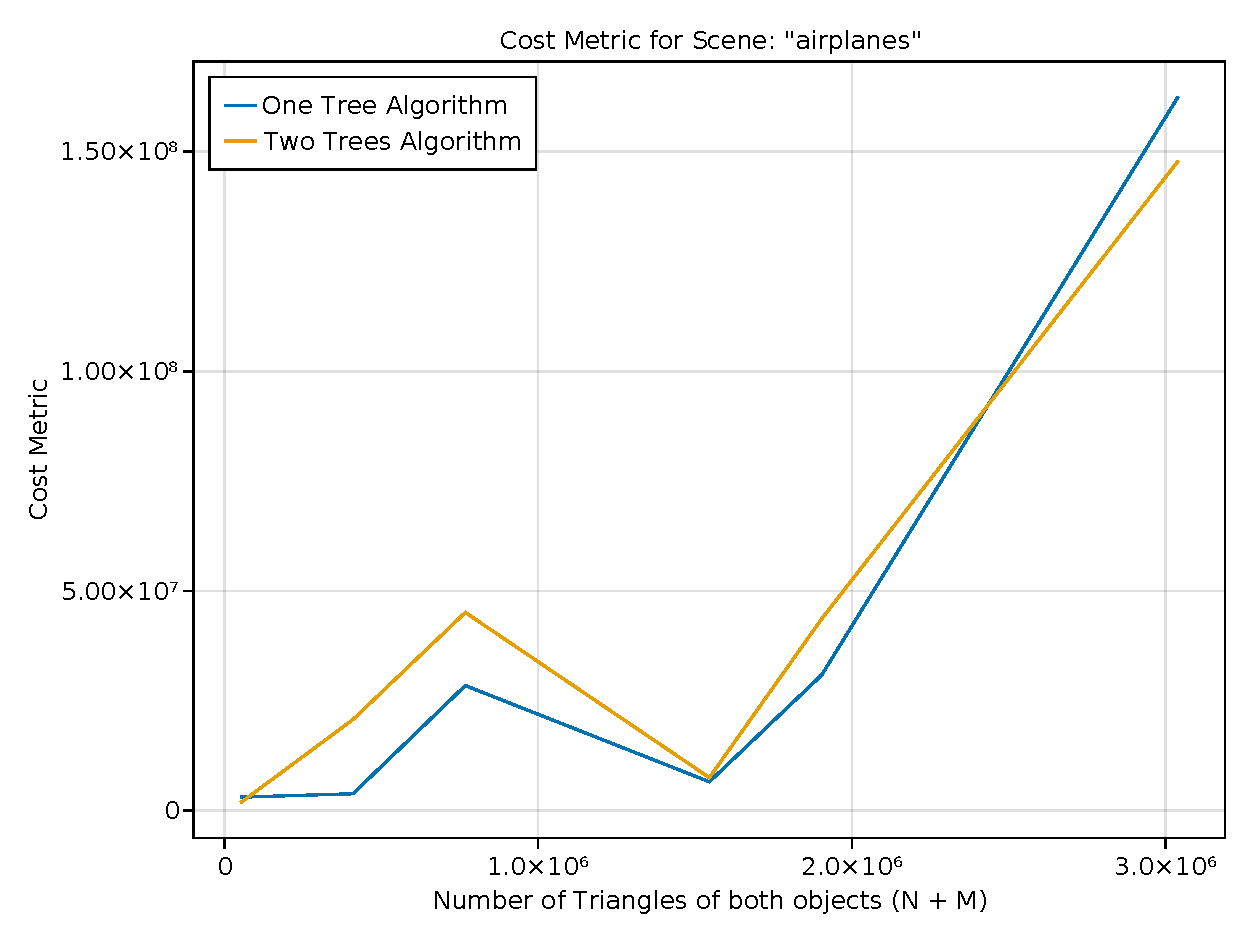
\includegraphics[width=0.6\textwidth]{cost_metric/airplanes_cost_metric.pdf}
    \caption[Κόστος Αναζήτησης για "αεροπλάνα"] {
        Κόστος αναζήτησης για τη σκηνή "αεροπλάνα" συναρτήσει 
        του μεγέθους των δύο μοντέλων.
    }
\end{figure}

\begin{figure}[H]
    \centering
    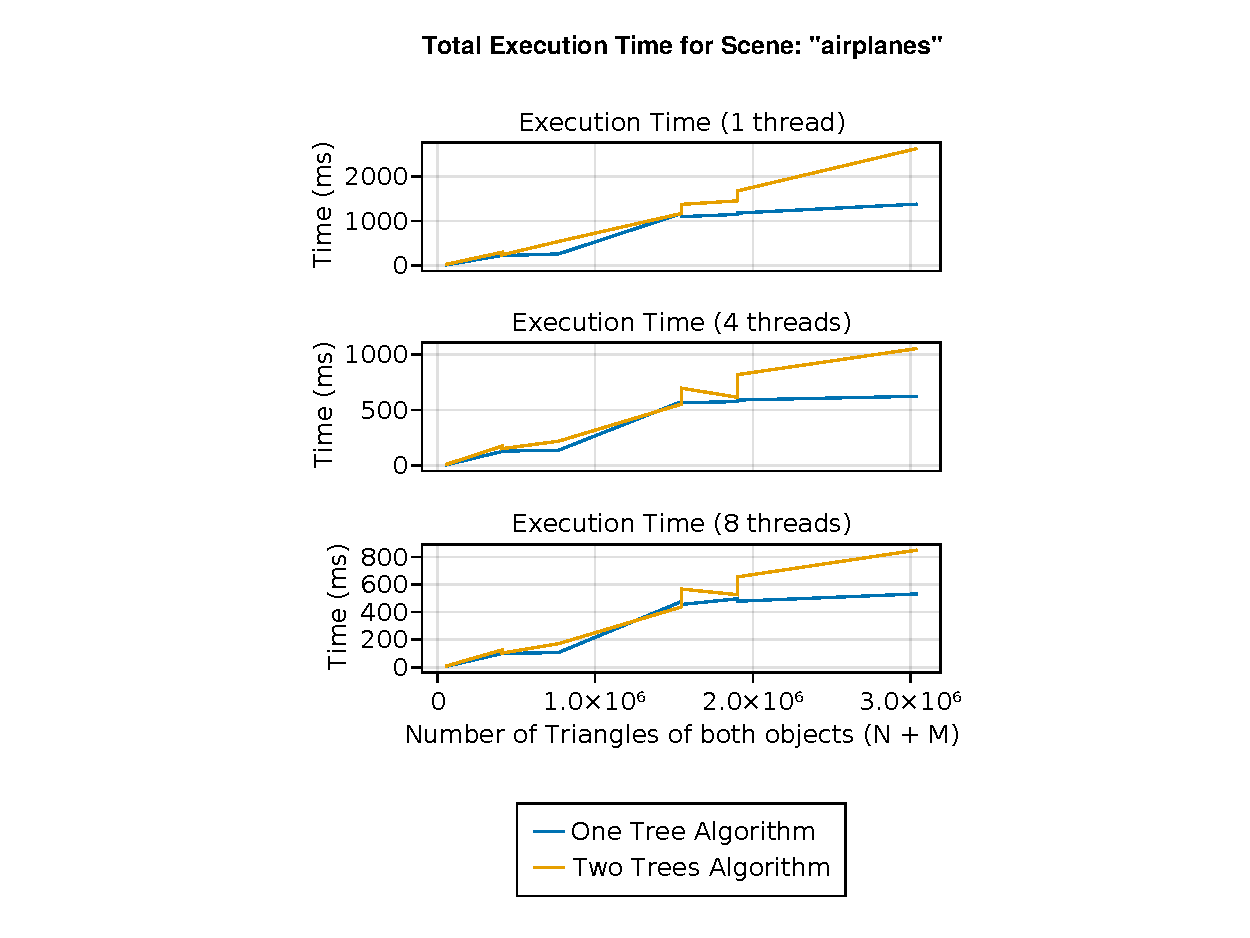
\includegraphics[width=1.0\textwidth]{execution_times/airplanes_exec_time.pdf}
    \caption[Συνολικός Χρόνος Εκτέλεσης για "αεροπλάνα"] {
        Συνολικός χρόνος εκτέλεσης ερωτήματος απόστασης 
        για τη σκηνή "αεροπλάνα" συναρτήσει του μεγέθους των δύο μοντέλων.
    }
\end{figure}

\subsection{\tl{Scooby} με \tl{Stanford Bunny}}
\begin{figure}[H]
    \centering
    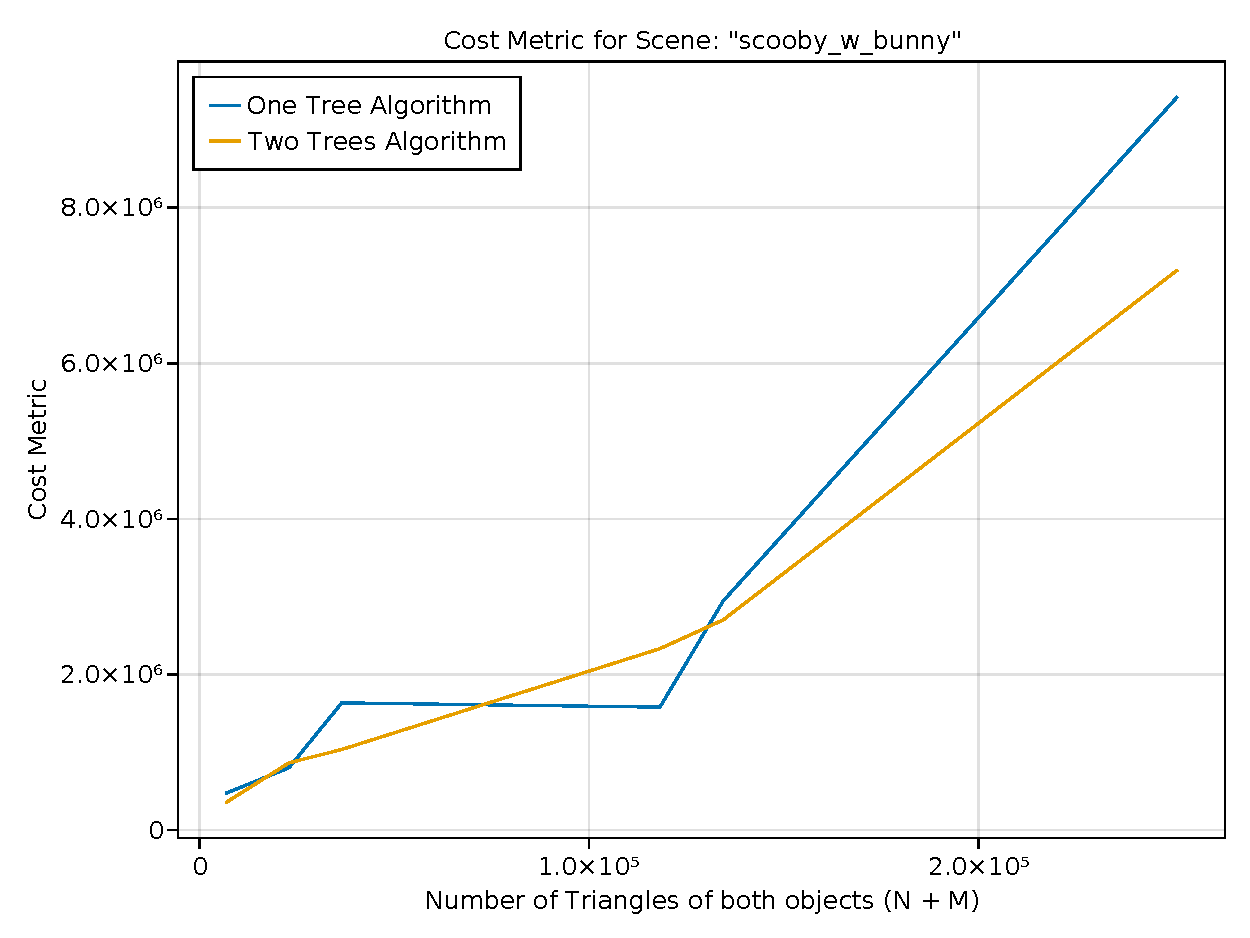
\includegraphics[width=0.6\textwidth]{cost_metric/scooby_w_bunny_cost_metric.pdf}
    \caption[Κόστος Αναζήτησης για "\tl{Scooby} με \tl{Stanford Bunny}"] {
        Κόστος αναζήτησης για τη σκηνή "\tl{Scooby} με \tl{Stanford Bunny}" συναρτήσει 
        του μεγέθους των δύο μοντέλων.
    }
\end{figure}

\begin{figure}[H]
    \centering
    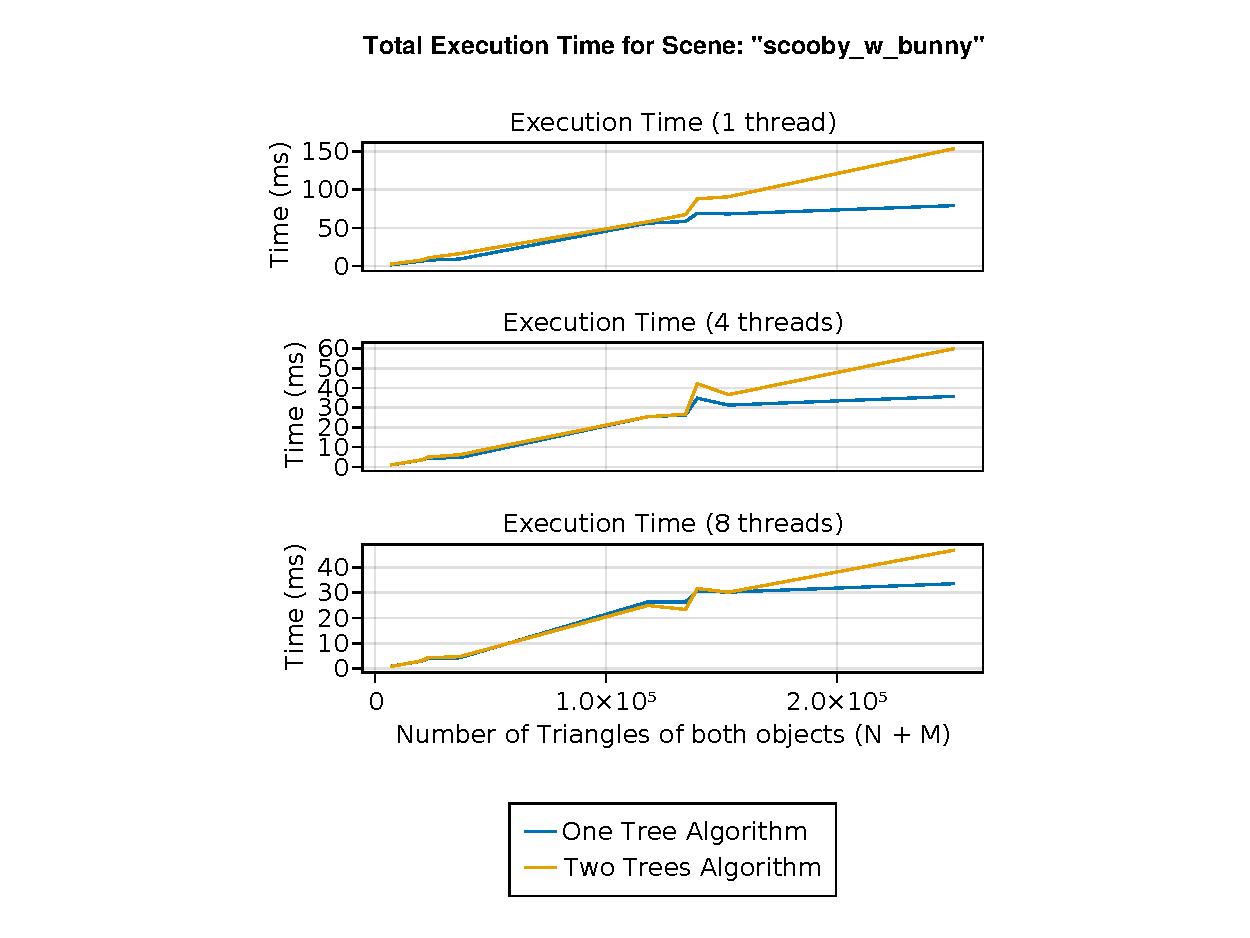
\includegraphics[width=1.0\textwidth]{execution_times/scooby_w_bunny_exec_time.pdf}
    \caption[Συνολικός Χρόνος Εκτέλεσης για "\tl{Scooby} με \tl{Stanford Bunny}"] {
        Συνολικός χρόνος εκτέλεσης ερωτήματος απόστασης 
        για τη σκηνή "\tl{Scooby} με \tl{Stanford Bunny}" συναρτήσει του μεγέθους των δύο μοντέλων.
    }
\end{figure}


\subsection{Ομοαξονικοί Κύλινδροι}
\begin{figure}[H]
    \centering
    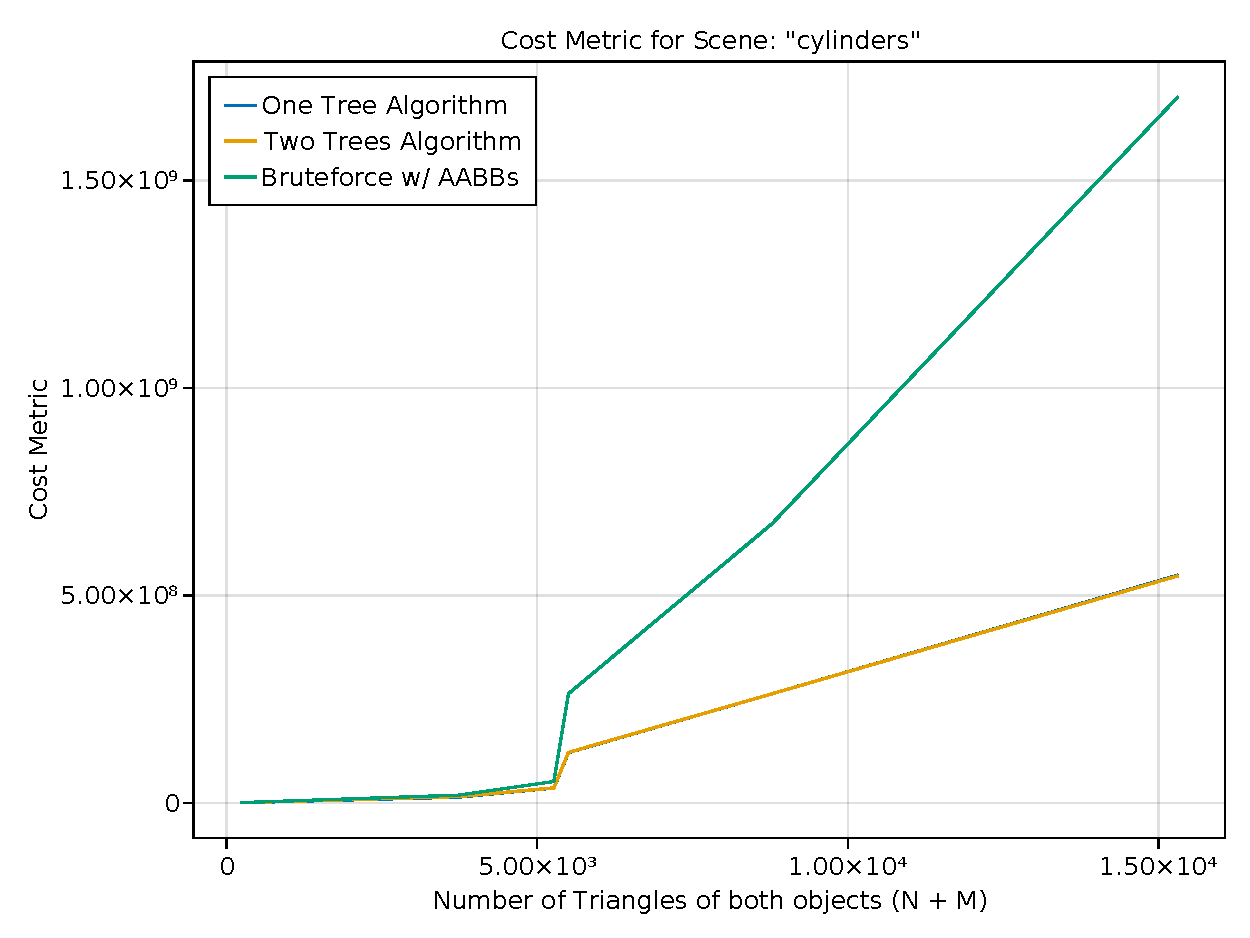
\includegraphics[width=0.6\textwidth]{cost_metric/cylinders_cost_metric.pdf}
    \caption[Κόστος Αναζήτησης για "ομοαξονικοί κύλινδροι"] {
        Κόστος αναζήτησης για τη σκηνή "ομοαξονικοί κύλινδροι" συναρτήσει 
        του μεγέθους των δύο μοντέλων.
    }
\end{figure}

\begin{figure}[H]
    \centering
    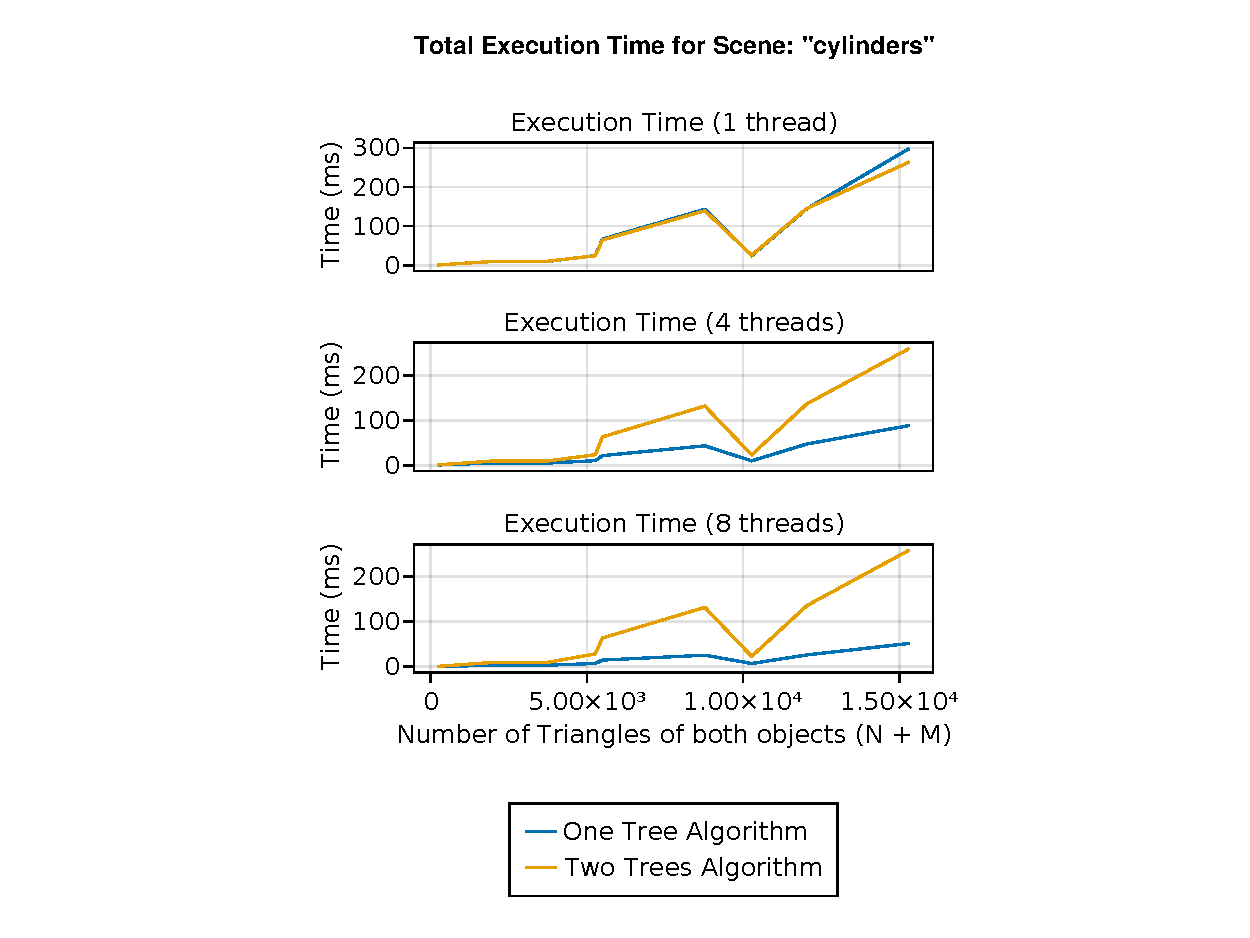
\includegraphics[width=1.0\textwidth]{execution_times/cylinders_exec_time.pdf}
    \caption[Συνολικός Χρόνος Εκτέλεσης για "ομοαξονικοί κύλινδροι"] {
        Συνολικός χρόνος εκτέλεσης ερωτήματος απόστασης 
        για τη σκηνή "ομοαξονικοί κύλινδροι" συναρτήσει του μεγέθους των δύο μοντέλων.
    }
\end{figure}


\subsection{Αλυσιδωτοί Τόροι}
\begin{figure}[H]
    \centering
    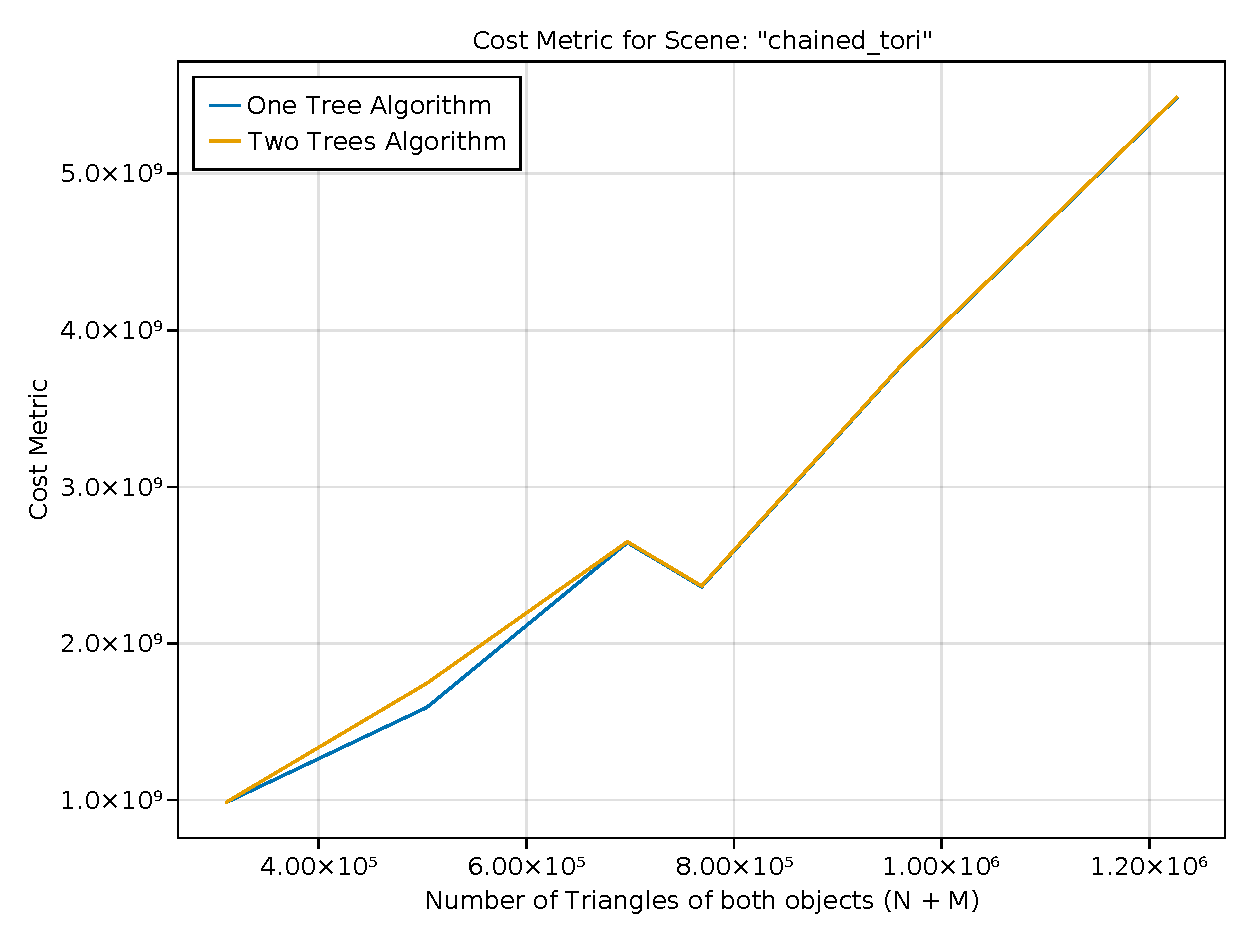
\includegraphics[width=0.6\textwidth]{cost_metric/chained_tori_cost_metric.pdf}
    \caption[Κόστος Αναζήτησης για "αλυσιδωτοί τόροι"] {
        Κόστος αναζήτησης για τη σκηνή "αλυσιδωτοί τόροι" συναρτήσει 
        του μεγέθους των δύο μοντέλων.
    }
\end{figure}

\begin{figure}[H]
    \centering
    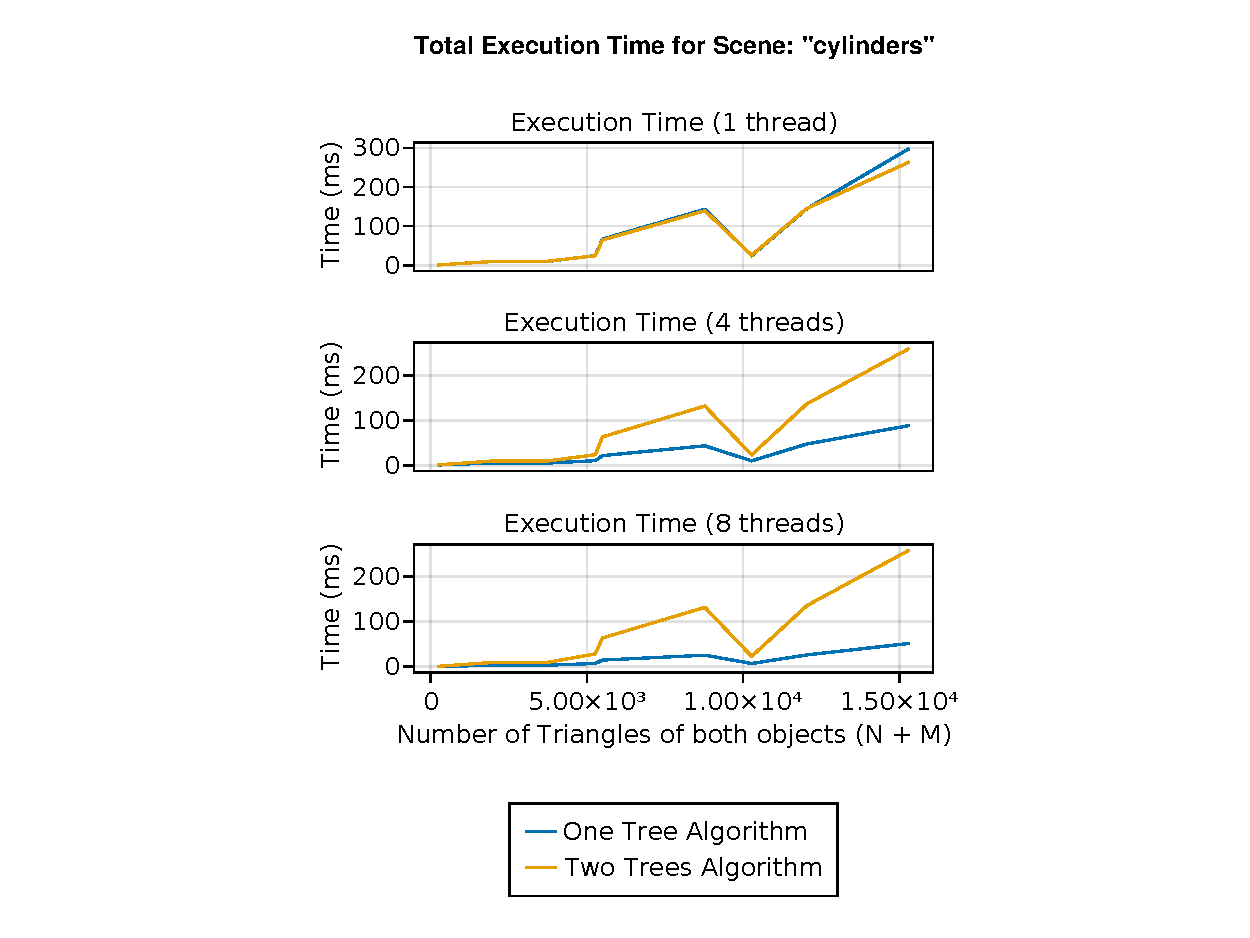
\includegraphics[width=1.0\textwidth]{execution_times/cylinders_exec_time.pdf}
    \caption[Συνολικός Χρόνος Εκτέλεσης για "ομοαξονικοί κύλινδροι"] {
        Συνολικός χρόνος εκτέλεσης ερωτήματος απόστασης 
        για τη σκηνή "ομοαξονικοί κύλινδροι" συναρτήσει του μεγέθους των δύο μοντέλων.
    }
\end{figure}

\subsection{Συγκρουόμενοι Τόροι}
\begin{figure}[H]
    \centering
    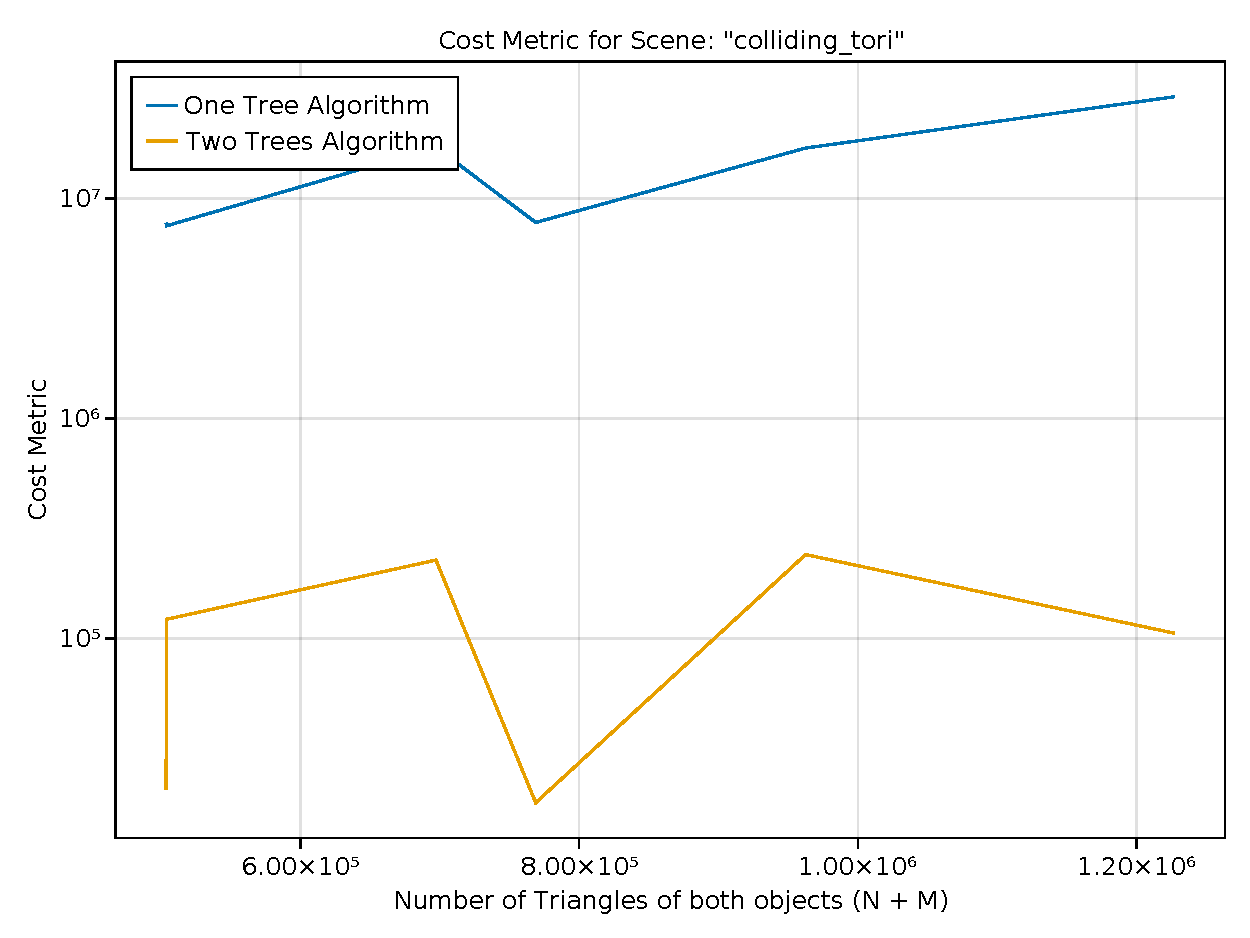
\includegraphics[width=0.6\textwidth]{cost_metric/colliding_tori_cost_metric.pdf}
    \caption[Κόστος Αναζήτησης για "συγκρουόμενοι τόροι"] {
        Κόστος αναζήτησης για τη σκηνή "συγκρουόμενοι τόροι" συναρτήσει 
        του μεγέθους των δύο μοντέλων.
    }
\end{figure}

\begin{figure}[H]
    \centering
    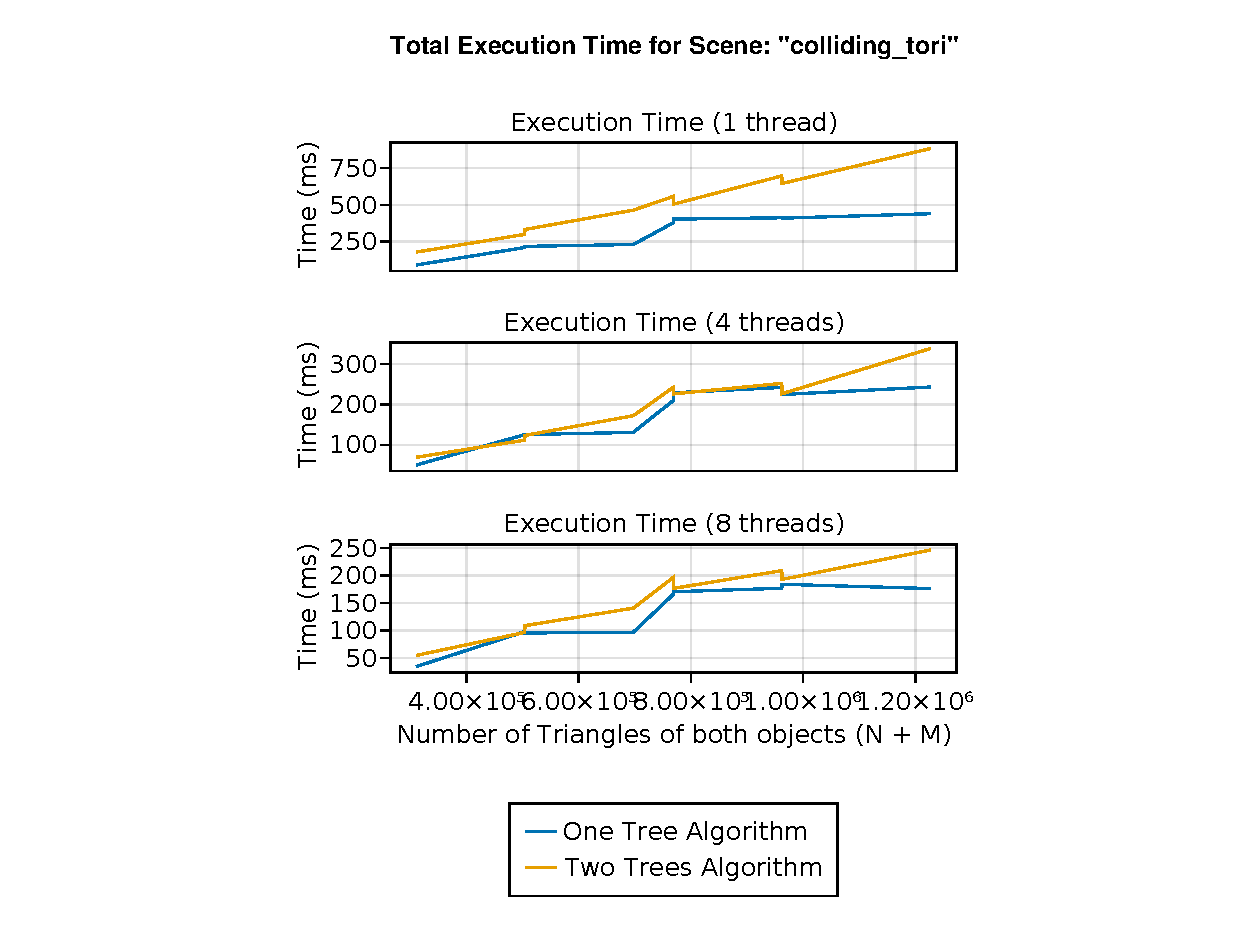
\includegraphics[width=1.0\textwidth]{execution_times/colliding_tori_exec_time.pdf}
    \caption[Συνολικός Χρόνος Εκτέλεσης για "συγκρουόμενοι τόροι"] {
        Συνολικός χρόνος εκτέλεσης ερωτήματος απόστασης 
        για τη σκηνή "συγκρουόμενοι τόροι" συναρτήσει του μεγέθους των δύο μοντέλων.
    }
\end{figure}


\section{Σχέση Απόστασης - Κόστους Αναζήτησης}
Για το πείραμα αυτό επιλέχθηκαν τα αντικείμενα της σκηνής 
"Αεροπλάνα" με περίπου $1.5 * 10^6$ τρίγωνα το καθένα.
Η αρχική θέση των αντικειμένων είναι αυτή που απεικονίζεται 
στην εικόνα \ref{fig:scenarios_photos}.
Έπειτα το ένα αεροπλάνο μετακινείται 
προς μια κατεύθυνση τέτοια ώστε να απομακρύνεται 
από το άλλο αεροπλάνο.

Στην εικόνα \ref{fig:cost_metric_vs_distance} 
σχεδιάζεται το κόστος αναζήτησης συναρτήσει της 
κανονικοποιημένης απόστασης των αντικειμένων, 
ενώ στην εικόνα \ref{fig:search_time_vs_distance} 
παρουσιάζεται ο χρόνος αναζήτησης (μόνο) συναρτήσει 
της κανονικοποιημένης απόστασης. 
Η απόσταση είναι κανονικοποιημένη και ίση με 
$\frac{dist}{diagonal}$, όπου $dist$ η πραγματική 
απόσταση των αντικειμένων και $diagonal$ το μήκος 
της διαγωνίου του \tl{AABB} του αεροπλάνου.


\begin{figure}[H]
    \centering
    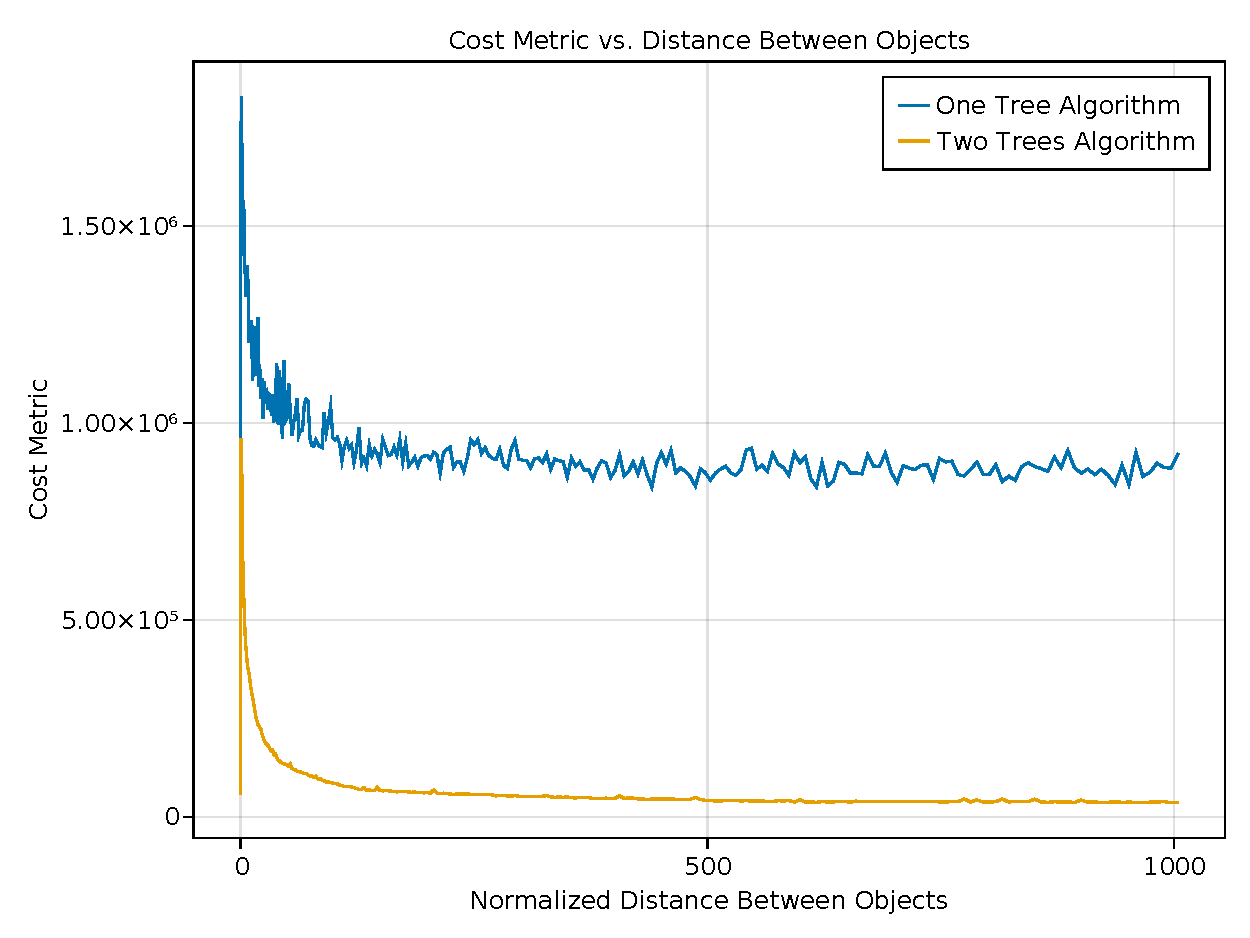
\includegraphics[width=0.6\textwidth]{cost_vs_distance.pdf}
    \caption[Κόστος Αναζήτησης Συναρτήσει της Απόστασης"] {
        Κόστος αναζήτησης συναρτήσει της απόστασης.
        Τα αντικείμενα ανήκουν στη σκηνή "αεροπλάνα".
    }
    \label{fig:cost_metric_vs_distance}
\end{figure}

\begin{figure}[H]
    \centering
    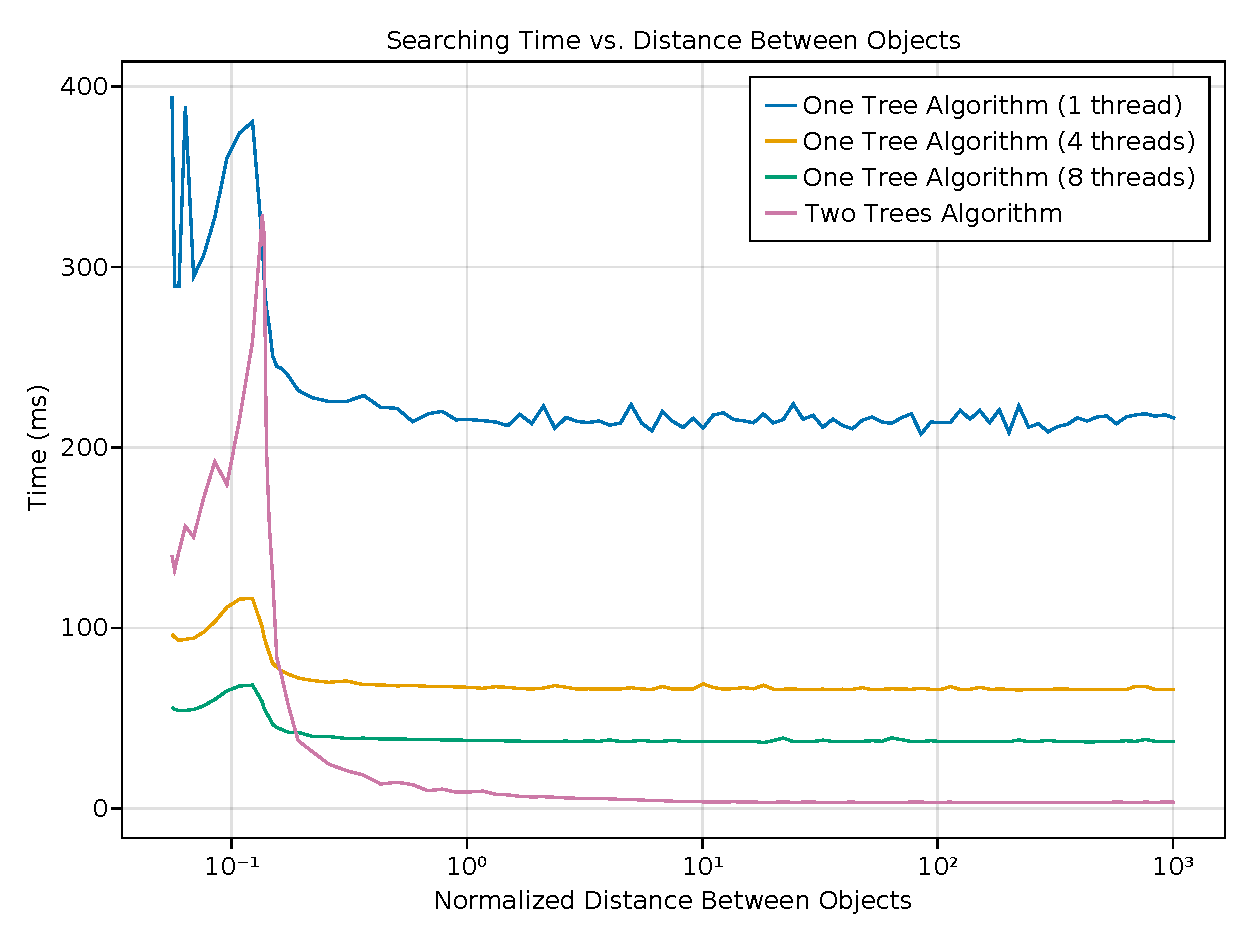
\includegraphics[width=0.6\textwidth]{search_time_vs_distance.pdf}
    \caption[Χρόνος Αναζήτησης Συναρτήσει της Απόστασης"] {
        Χρόνος αναζήτησης συναρτήσει της απόστασης.
        Τα αντικείμενα ανήκουν στη σκηνή "αεροπλάνα".
        \textit{Σημείωση}: Ο αλγόριθμος που χρησιμοποιεί δύο \tl{sKD-Trees} δεν 
        είναι παράλληλος.
    }
    \label{fig:search_time_vs_distance}
\end{figure}




% να προσθέσω ποσοστά χρόνου αναζήτησης/κατασκευής

\chapter{Επίλογος}
\label{ch:conclusion}
Σε αυτή τη διπλωματική εργασία μελετήσαμε το πρόβλημα εύρεσης της 
Ευκλείδειας απόστασης δύο τριγωνικών πλεγμάτων.

Στη μεθοδολογία που ακολουθήσαμε, σχεδιάσαμε μια δομή δεδομένων που 
ανήκει στην οικογένεια των Ιεραρχιών Οριοθετικών Όγκων, το \tl{sKD-Tree}, 
και προτείναμε δύο αλγορίθμους που κάνουν χρήση αυτής της δομής.
Οι αλγόριθμοι που σχεδιάσαμε γενικεύονται και για άλλα ήδη πλεγμάτων 
πέραν των τριγωνικών, υπό τις προϋποθέσεις που στο κεφάλαιο \ref{ch:methodology}.
Στη συνέχεια παρουσιάσαμε τα αποτελέσματα της εφαρμογής των αλγορίθμων 
μας σε μια σειρά από σενάρια ελέγχου που κατασκευάσαμε.
Με τα παραπάνω αποτελέσματα περιγράφουμε την επίδοση 
των αλγορίθμων ανά σενάριο, και ταυτόχρονα κάνουμε τη σύγκριση μεταξύ 
τους.

Σε αυτό το κεφάλαιο, θα σχολιάσουμε τα αποτελέσματα και θα προτείνουμε 
τη μελλοντική εργασία που μπορεί να επεκτείνει την παρούσα διπλωματική 
εργασία.

\section{Συμπεράσματα}
Ξεκινώντας από το διάγραμμα του σχήματος \ref{fig:build_time} με τους 
χρόνους κατασκευής του \tl{sKD-Tree} παρατηρούμε ότι η διαδικασία 
της κατασκευής δεν μπορεί να επιταχυνθεί γραμμικά σε σχέση με το πλήθος 
των νημάτων που χρησιμοποιούνται.
Αυτό προκύπτει από το γεγονός ότι δεν μπορούμε να εκμεταλλευτούμε όλα τα 
νήματα από την αρχή.
Συγκεκριμένα για κάθε κόμβο του δέντρου πρώτα γίνεται ο διαχωρισμός 
των τριγώνων σε δύο υποσύνολα, το οποίο γίνεται σειριακά,
και έπειτα η κατασκευή του αριστερού και δεξιού παιδιού παράλληλα.
Επομένως, για την κατασκευή της ρίζας μπορούμε να εκμεταλλευτούμε
μόνο δύο νήματα, ενώ για το δεύτερο επίπεδο του δέντρου μόνο 4 και 
ούτω καθεξής. 
Έτσι τα νήματα παραμένουν αδρανή στα πρώτα επίπεδα χτισίματος του 
δέντρου.
Επίσης, παρατηρούμε ότι η επιπλέον επιτάχυνση που επιτυγχάνεται 
για κάθε επιπλέον νήμα που προστίθεται είναι όλο και μικρότερη 
(πίνακας \ref{tab:build_acceleration}). 

\begin{table}[h]
    \centering
    \begin{tabular}{|c|c|c|c|c|}
        \hline 
         & 1 \tl{thread} & 2 \tl{threads} & 4 \tl{threads} & 8 \tl{threads} \\
        \hline
        Επιτάχυνση & $\times1$ & $\times 1.40$ & $\times 1.92$ & $\times 2.14$ \\
        \hline
    \end{tabular}
    \caption[]{Επιτάχυνση κατασκευής του \tl{sKD-Tree} συναρτήσει των νημάτων}
    \label{tab:build_acceleration}
\end{table}

Σύμφωνα με τα παραπάνω, και για τα μεγέθη των πλεγμάτων που χρησιμοποιήθηκαν, 
ο χρόνος κατασκευής του δέντρου με τέσσερα νήματα, πρακτικά, δε διαφέρει 
από τον χρόνο κατασκευής με οκτώ. 
Με αφορμή αυτή την παρατήρηση και το γεγονός ότι ο αλγόριθμος \ref{alg:queries_on_tree}
έχει έναν παράγοντα τυχαιότητας, σχεδιάσαμε τον αλγόριθμο \ref{alg:search_on_two_trees}
που χρησιμοποιεί δύο \tl{sKD-Tree}.
Ο αλγόριθμος αυτός εκτελεί την αναζήτηση με συγκεκριμένη σειρά, οπότε δεν είναι τυχαίος,
ενώ η προεπεξεργασία μπορεί να πραγματοποιηθεί στον ίδιο, πρακτικά, χρόνο εάν τα 
δύο δέντρα κατασκευαστούν παράλληλα.

Στόχος του αλγορίθμου \ref{alg:search_on_two_trees} ήταν να επιτυγχάνει πολύ 
μικρό κόστος αναζήτησης. 
Ιδανικά μια διάσχιση του πρώτου δέντρου και μια του δεύτερου, δηλαδή πολυπλοκότητα 
της τάξης $\bigO(log(N) + log(M))$ ή $\bigO(log(N) * log(M))$ στη 
μέση περίπτωση.
Ο αλγόριθμος \ref{alg:search_on_two_trees} επιτυγχάνει αρκετά μικρότερο κόστος 
αναζήτησης από τον \ref{alg:queries_on_tree} μόνο στις περιπτώσεις 
που τα αντικείμενα συγκρούονται ή όταν απέχουν αρκετά.
Όμως, ακόμη και σε αυτές τις περιπτώσεις, η διαφορά στο χρόνο αναζήτησης 
δεν είναι μεγάλη, καθώς για τα σενάρια μας αυτή 
ήταν από $50ms$ έως $200ms$ (σχήμα \ref{fig:search_time_vs_distance}).
Σε όλες τις άλλες περιπτώσεις το κόστος αναζήτησης του αλγορίθμου 
\ref{alg:search_on_two_trees} ήταν χειρότερο από αυτό του \ref{alg:queries_on_tree}.
Επιπλέον, από τα διαγράμματα του κεφαλαίου \ref{sec:profiling} προκύπτει τελικά 
ότι το ποσοστό του χρόνου αναζήτησης για τον αλγόριθμο \ref{alg:queries_on_tree}
είναι μικρό (περίπου $6\% - 15\%$) στη μέση περίπτωση.
Επομένως, εξίσου μικρά είναι και τα περιθώρια βελτίωσης του χρόνου αναζήτησης.

Τελικά, με βάση όλα όσα αναφέρθηκαν παραπάνω, ο αλγόριθμος \ref{alg:queries_on_tree} 
που χρησιμοποιεί ένα \tl{sKD-Tree} και εκτελεί παράλληλα ερωτήματα κοντινότερου 
γείτονα φαίνεται να είναι ο προτιμότερος.


\section{Μελλοντική Εργασία}

\appendix
\chapter{Ακρωνύμια και συντομογραφίες}

\selectlanguage{english}
\begin{description}
  \item[AABB] Axis-Aligned Bounding Box
  \item[BVH] Bounding Volume Hierarchy
  \item[CAE] Computer Aided Engineering
  \item[DFS] Depth First Search
\end{description}
\selectlanguage{greek}


\selectlanguage{english}

\bibliography{references}{}
\bibliographystyle{abbrv}

\end{document}